\documentclass[12pt,oneside,openright]{report}

% Page layout and formatting
\usepackage[a4paper,margin=1in,bindingoffset=0.5cm,headheight=15pt]{geometry}
\usepackage{setspace}
\onehalfspacing % More professional than double spacing

% Paragraph formatting: Remove indentation and add vertical space between paragraphs
\setlength{\parindent}{0pt}
\setlength{\parskip}{1em}

% Font and encoding (modern approach)
\usepackage[utf8]{inputenc}
\usepackage[T1]{fontenc}
\usepackage{lmodern}
\usepackage{microtype} % Improved typography
% Relax line-breaking to avoid overfull hboxes in math-heavy paragraphs
\emergencystretch=1.5em

% Mathematics and physics
\usepackage{amsmath, amssymb, amsthm}
\usepackage{siunitx}
\usepackage{physics}
% Ensure \qty uses siunitx definition to avoid package clash warning
\AtBeginDocument{\RenewCommandCopy\qty\SI}
\usepackage{mathtools}
\usepackage{bm} % Bold math symbols

% Graphics and figures
\usepackage{graphicx}
\usepackage{float}
\usepackage{subcaption}
\usepackage{tikz}
\usepackage{pgfplots}
\pgfplotsset{compat=1.18}
\usetikzlibrary{arrows.meta,positioning,calc}

% Tables
\usepackage{booktabs}
\usepackage{array}
\usepackage{longtable}
\usepackage{multirow}

% Code listings
\usepackage{listings}
\lstset{
  language=Python,
  basicstyle=\ttfamily\small,
  keywordstyle=\color{blue}\bfseries,
  stringstyle=\color{red!70!black},
  commentstyle=\color{green!50!black}\itshape,
  numbers=left,
  numberstyle=\tiny\color{gray},
  numbersep=5pt,
  breaklines=true,
  breakatwhitespace=true,
  frame=single,
  framesep=3pt,
  tabsize=4,
  showstringspaces=false,
  columns=flexible,
  aboveskip=10pt,
  belowskip=10pt,
  xleftmargin=2em,
  framexleftmargin=1.5em,
}

% Professional enhancements
\usepackage{xcolor}
\definecolor{linkcolor}{RGB}{0,0,139}
\definecolor{citecolor}{RGB}{139,0,0}
\definecolor{urlcolor}{RGB}{0,139,0}

% Citations and bibliography (modern biblatex setup)
\usepackage[style=phys,backend=biber,sorting=none,maxbibnames=99]{biblatex}
\addbibresource{references.bib}

% Professional headers and footers
\usepackage{fancyhdr}
\pagestyle{fancy}
\fancyhf{}
\fancyhead[R]{\thepage}
\fancyhead[L]{\nouppercase{\leftmark}}
\renewcommand{\headrulewidth}{0.3pt}
\renewcommand{\footrulewidth}{0pt}

% Chapter and section formatting
\usepackage{titlesec}
\titleformat{\chapter}[display]
  {\normalfont\huge\bfseries}{\chaptertitlename\ \thechapter}{20pt}{\Huge}
\titlespacing*{\chapter}{0pt}{0pt}{40pt}

% Caption formatting
\usepackage{caption}
\captionsetup{format=plain,labelfont=bf,textfont=normal,justification=justified,singlelinecheck=false}

% Hyperlinks and PDF properties (load near end)
\usepackage[colorlinks=true,linkcolor=linkcolor,citecolor=citecolor,urlcolor=urlcolor,
            bookmarks=true,bookmarksnumbered=true,pdfstartview=FitH]{hyperref}
\usepackage{bookmark}

% Professional theorem environments
\theoremstyle{definition}
\newtheorem{definition}{Definition}[chapter]

\theoremstyle{plain}
\newtheorem{theorem}{Theorem}[chapter]
\newtheorem{lemma}[theorem]{Lemma}
\newtheorem{proposition}[theorem]{Proposition}
\newtheorem{corollary}[theorem]{Corollary}

\theoremstyle{remark}
\newtheorem{remark}{Remark}[chapter]
\newtheorem{example}{Example}[chapter]

% Custom commands for physics notation (only add commands not in physics package)
% Note: physics package already provides \ket, \bra, \braket, \tr
\newcommand{\avg}[1]{\left\langle#1\right\rangle}

% Equation shortcuts
\newcommand{\beq}{\begin{equation}}
\newcommand{\eeq}{\end{equation}}

% SI units configuration
\sisetup{
  per-mode=symbol,
  range-phrase=--,
  range-units=single,
  detect-weight=true,
  detect-family=true
}

% PDF metadata
\hypersetup{
    pdftitle={Page Curve Like Entanglement Dynamics in Many-Body Quantum Systems},
    pdfauthor={Prosanto Bhakta},
    pdfsubject={Theoretical Physics - Quantum Many-Body Systems},
    pdfkeywords={quantum entanglement, many-body systems, Page curve, fermionic systems, resonant level model, correlation matrix}
}

% Title page information
\title{Page Curve Like Entanglement Dynamics in Many-Body Quantum Systems: \\
A Study of a Free Fermionic Model}
\author{Prosanto Bhakta}
\date{26 February 2026}

\begin{document}
% Avoid duplicate page anchors for front matter
\hypersetup{pageanchor=false}

% Professional title page
\begin{titlepage}
\setlength{\parskip}{0pt}% Reset parskip for title page only
\centering
\small

\vspace*{-1.5cm}

% University logo pushed to the very top

\includegraphics[width=7cm, trim=150 80 150 300, clip]{figures/iub_logo.png}

\vspace{-1.5cm}

{\normalsize\textsc{Independent University, Bangladesh}\\[0.2cm]
\small\textsc{Department of Physical Sciences}}

\vspace{0.8cm}

{\Large\bfseries Page Curve Like Entanglement Dynamics in\\[0.2cm]
Many-Body Quantum Systems:\\[0.2cm]
A Study of a Free Fermionic Model\par}

\vspace{0.6cm}

{\normalsize\textsc{PHY499 -- Project in Physics}\par}

\vspace{0.6cm}
{\normalsize\textsc{A thesis submitted in partial fulfillment of the\\[0.2cm]
requirements for the degree of}\\[0.3cm]
\large\textbf{Bachelor of Science in Physics}\par}

\vspace{0.4cm}

{\large\textsc{by}}

\vspace{0.2cm}

{\large\textbf{Prosanto Bhakta}\\[0.2cm]
\normalsize Student ID: 2010271}

\vspace{0.4cm}

{\large\textsc{Supervisor:}\\[0.1cm]
\textbf{M. Arshad Momen}\\[0.1cm]
\textit{Professor}\\[0.1cm]
\textit{Department of Physical Sciences}}

\vfill

{\large February 2026}

\vspace{1cm}

\end{titlepage}

% Front matter
% Note: report class doesn't have \frontmatter, so we'll use manual page numbering
\pagenumbering{roman}

% Declaration
\chapter*{Declaration}

I, Prosanto Bhakta, hereby declare that the thesis titled
\textit{Page Curve Like Entanglement Dynamics in Many-Body Quantum Systems: A Study of a Free Fermionic Model}
is my own original work, carried out under the supervision of Professor M. Arshad Momen,
Department of Physical Sciences, Independent University, Bangladesh.

I further declare that this work, in whole or in part, has not been previously submitted
for any degree or diploma at this or any other institution.
No other sources or learning aids, other than those listed in this thesis, have been used.
Furthermore, I declare that I have acknowledged the work of others by providing detailed references to all such work.

\vspace{2cm}

\noindent\begin{minipage}[t]{0.48\textwidth}
\textbf{Signature of the student:}\\[1.2cm]
\end{minipage}\hfill
\begin{minipage}[t]{0.40\textwidth}
\rule{0.9\linewidth}{0.4pt}
\end{minipage}

\cleardoublepage



% Certification of The Report
\chapter*{Certification of The Report}

The report titled
\textit{Page Curve Like Entanglement Dynamics in Many-Body Quantum Systems: A Study of a Free Fermionic Model}
submitted by \textbf{Prosanto Bhakta} (Student ID: 2010271)
has been accepted as satisfactory in partial fulfillment of the requirements for the degree of
BSc (Hons.) in Physics on 26th February 2026.

\vspace{1cm}

\noindent\textbf{Members of the Assessment Committee:}

\vspace{0.5cm}

\noindent\begin{minipage}[t]{0.62\textwidth}
\textbf{M. Arshad Momen, PhD}\\
Dept. of Physical Sciences\\
\textit{Supervisor}
\end{minipage}\hfill
\begin{minipage}[t]{0.34\textwidth}
\rule{\linewidth}{0.4pt}
\end{minipage}

\vspace{0.6cm}

\noindent\begin{minipage}[t]{0.62\textwidth}
\textbf{Ahmad Mostofa Kamal, PhD}\\
Dept. of Physical Sciences\\
\textit{Member}
\end{minipage}\hfill
\begin{minipage}[t]{0.34\textwidth}
\rule{\linewidth}{0.4pt}
\end{minipage}

\vspace{0.6cm}

\noindent\begin{minipage}[t]{0.62\textwidth}
\textbf{Farhad Alam, PhD}\\
Dept. of Physical Sciences\\
\textit{Member}
\end{minipage}\hfill
\begin{minipage}[t]{0.34\textwidth}
\rule{\linewidth}{0.4pt}
\end{minipage}

\vspace{0.6cm}

\noindent\begin{minipage}[t]{0.62\textwidth}
\textbf{Jewel Kumar Ghosh, PhD}\\
Dept. of Physical Sciences\\
\textit{Member}
\end{minipage}\hfill
\begin{minipage}[t]{0.34\textwidth}
\rule{\linewidth}{0.4pt}
\end{minipage}

\vspace{0.6cm}

\noindent\begin{minipage}[t]{0.62\textwidth}
\textbf{Rifat Ara Rouf, PhD}\\
Dept. of Physical Sciences\\
\textit{Head of the Department}
\end{minipage}\hfill
\begin{minipage}[t]{0.34\textwidth}
\rule{\linewidth}{0.4pt}
\end{minipage}




\cleardoublepage

% Approval
\chapter*{Approval}

This is to certify that the thesis titled
\textit{Page Curve Like Entanglement Dynamics in Many-Body Quantum Systems: A Study of a Free Fermionic Model},
submitted by Prosanto Bhakta (Student ID: 2010271), has been examined and approved
as partial fulfillment of the requirements for the degree of Bachelor of Science in Physics,
Department of Physical Sciences, Independent University, Bangladesh.

\vspace{2cm}

\noindent\begin{minipage}[t]{0.62\textwidth}
\textbf{Signature of the Supervisor:}\\

\end{minipage}\hfill
\begin{minipage}[t]{0.34\textwidth}
\rule{\linewidth}{0.4pt}
\end{minipage}

\vspace{0.8cm}

\noindent\begin{minipage}[t]{0.62\textwidth}
\textbf{Signature of the Head of the Department:}\\
\end{minipage}\hfill
\begin{minipage}[t]{0.34\textwidth}
\rule{\linewidth}{0.4pt}
\end{minipage}

\vspace{0.8cm}

\noindent\begin{minipage}[t]{0.62\textwidth}
\textbf{Signature of the Director, GSRIR:}\\

\end{minipage}\hfill
\begin{minipage}[t]{0.34\textwidth}
\rule{\linewidth}{0.4pt}
\end{minipage}

\vspace{1.5cm}


\cleardoublepage

% Abstract
\chapter*{Abstract}
\addcontentsline{toc}{chapter}{Abstract}

This thesis investigates entanglement dynamics in open quantum many-body systems, focusing on a one-dimensional free-fermion model in which a finite system is coupled to a large environment. We study the model introduced in Ref.~\cite{Kehrein_2024}, which becomes exactly solvable in the weak-coupling limit. Using resonant-level-model factorization, we derive analytical expressions for the entanglement dynamics and validate them with numerical simulations based on the correlation matrix formalism. We show that the system exhibits Page-curve-like behavior: the entanglement entropy grows at early times, reaches a maximum at the Page time (proportional to system size), and then decreases at late times. In the appropriate scaling regime, data for different system sizes collapse onto a single curve when plotted against the emitted-particle fraction. These results provide an analytically controlled and numerically validated framework for understanding Page-curve dynamics in open free-fermion systems.

\cleardoublepage

% Dedication
\chapter*{Dedication}

\vspace*{0.25\textheight}
\begin{center}
{\Large\itshape
To my father,\\
who devoted his life to our education.\\
Though you are no longer here,\\
this achievement is yours as much as mine.}
\end{center}

\cleardoublepage


\chapter*{Acknowledgments}
\addcontentsline{toc}{chapter}{Acknowledgments}

I would like to express my deepest gratitude to my supervisor, Professor M. Arshad Momen,
for his invaluable guidance, patience, and unwavering support throughout this research journey.
I am grateful to the faculty members of the Department of Physical Sciences at Independent University, Bangladesh,
for providing an excellent academic environment and for their constructive feedback during various presentations of this work.
I acknowledge the computational resources provided by the Center for Computational and Data Sciences (CCDS) that enabled the numerical simulations presented in this work.
Finally, I would like to thank my family, especially my mother and sister, for their constant love, encouragement, and sacrifices, without which this achievement would not have been possible. I am also sincerely grateful to Mollika for her love and understanding.


% Table of contents with proper formatting
\renewcommand{\contentsname}{Table of Contents}
\tableofcontents
\addcontentsline{toc}{chapter}{Table of Contents}
\cleardoublepage

\listoffigures
\addcontentsline{toc}{chapter}{List of Figures}
\cleardoublepage


% Main matter
% Note: report class doesn't have \mainmatter, so we'll reset page numbering manually
\cleardoublepage
\hypersetup{pageanchor=true}
\pagenumbering{arabic}

% Main content
\chapter{Introduction}
\label{ch:introduction}

Quantum entanglement is a defining feature of quantum physics and has no classical analog.
First highlighted by Einstein, Podolsky, and Rosen in 1935~\cite{EPR1935}, and later named by Schrödinger~\cite{Schrodinger1935}, it describes correlations that cannot be captured by product-state descriptions of subsystems.
In an entangled state, the full system may be pure while each subsystem requires a reduced-state description.

Entanglement now plays a central role across modern physics.
In quantum information science, it is a resource for computation, cryptography, and teleportation~\cite{NielsenChuang}.
In condensed matter, entanglement entropy probes quantum phase transitions and topological order~\cite{Amico2008,Eisert2010}.
In high-energy physics, it is closely connected to holography and AdS/CFT~\cite{Ryu2006,VanRaamsdonk2010}.
In this thesis, entanglement entropy is our primary diagnostic, and we use it to analyze the dynamics of an analytically tractable fermionic model.

\section{The Page Curve}

An important qualitative feature of entanglement dynamics is the so-called Page curve.
It describes an entanglement entropy that first grows in time, reaches a maximum (the Page time), and then decreases as the subsystem loses accessible degrees of freedom.

This behavior was first discussed by Page~\cite{Page1993} in the context of black hole evaporation.
In 1974, Hawking showed that black holes emit thermal radiation due to quantum effects near the event horizon~\cite{Hawking1975}.
If this radiation were exactly thermal, it would carry no information about the initial state, creating a tension with unitarity.
Page showed that under unitary evaporation, the entanglement entropy between radiation and the remaining black hole must follow a rise-and-fall trajectory.

Recent developments involving the ``island formula'' have shown how semiclassical gravity can reproduce the Page curve~\cite{Penington2020,Almheiri2019,Almheiri2020}.
However, similar dynamics also appear in much simpler quantum many-body systems, which is the focus of this thesis.

\section{Page Curves in Many-Body Systems}

While the Page curve originated in black hole physics, similar behavior arises in simpler quantum many-body systems.
When a finite subsystem is coupled to a large environment, particles can leak from the subsystem into the bath.
The entanglement entropy typically grows during this process; if evolution is unitary and the subsystem eventually empties, the entropy must later decrease, producing Page-curve-like dynamics.

Studying Page curves in solvable many-body models offers several advantages:
they provide tractable settings where full entanglement dynamics can be computed with controlled approximations;
they help isolate universal Page-curve features beyond gravity-specific details;
and they can be connected to laboratory platforms such as ultracold atoms or trapped ions.

Recent work has explored Page-curve-like dynamics in random unitary circuits~\cite{Nahum2017}, integrable spin chains~\cite{Alba2017}, and free-fermion systems coupled to baths~\cite{Kehrein_2024}.
Models that become exactly solvable in controlled limits are particularly valuable because they allow detailed analytical understanding of the mechanisms that generate Page-curve behavior.

\section{This Thesis}

We investigate Page-curve-like entanglement dynamics in a one-dimensional free-fermion model where a finite system is coupled to a large environment.
The model, introduced in Ref.~\cite{Kehrein_2024}, describes a finite fermionic chain coupled to semi-infinite leads and becomes exactly solvable in the weak-coupling limit.

Our approach combines analytical and numerical methods.
Analytically, we use resonant-level-model factorization to decompose the many-body problem into independent single-particle channels.
Numerically, we apply the Peschel correlation-matrix formalism~\cite{Peschel_2003} to compute entanglement entropy efficiently.
Agreement between the two approaches validates the analytical predictions and reveals universal scaling: when plotted against the fraction of emitted particles, results for different system sizes collapse onto a single curve.

The thesis is organized as follows. Chapter~\ref{ch:theory} develops the theoretical background---density matrices, reduced density matrices, entanglement entropy, and second quantization. Chapter~\ref{ch:fermionic} presents the fermionic model, derives the analytical solution, and compares it with numerical simulations. Chapter~\ref{ch:conclusion} summarizes our findings and discusses extensions to interacting and bosonic systems.


\chapter{Theoretical Background}
\label{ch:theory}
We begin with the density matrix formalism in quantum mechanics and then extend the discussion to quantum entanglement within the same framework.
We also give a brief review of second quantization, which is the natural language for many-body quantum systems.
We then show how the notion of entropy is extended to entanglement entropy, interpreted here as a measure of quantum entanglement.
To do so, we distinguish pure and mixed states and describe both using density operators.
Density operators (density matrices) are central tools for expressing entropy for mixed states and for pure but entangled bipartite states.


\section{Density matrix formalism}
\label{sec:density_matrix}
In this thesis, we are primarily interested in subsystems.
Because one typically has access to only partial information about the full system, the density matrix is the appropriate description.
In quantum mechanics, the state of a system is commonly represented by a wavefunction $\psi$,
which encodes complete information about the system. However, this description becomes 
insufficient when the system is part of a larger ensemble, or when only partial information about its preparation is available.
In such cases, one must adopt a more general formalism that can describe both complete and incomplete knowledge of a system’s state.
This leads naturally to the density matrix (or density operator) formalism, which provides a unified framework for representing 
both pure and mixed quantum states.

Throughout this thesis, we work in natural units where $\hbar = 1$. This simplifies the notation for time evolution and commutation relations.

The density matrix is defined as 
\begin{equation}{\label{eq:density_matrix}}
\rho \equiv \sum_{i} p_i \ket{\psi_i} \bra{\psi_i}
\end{equation}
where the sum runs over all states in the ensemble, each $\ket{\psi_i}$ is a possible pure state of the system, and $p_i$ denotes the probability of
finding the system in that state. This construction allows us to treat statistical ensembles and individual quantum systems on the same footing.

\textbf{Properties of the density matrix}:
\begin{itemize}
\item \textbf{Hermiticity}: The density matrix is Hermitian, i.e. $\rho = \rho^{\dagger}$.
\item \textbf{Trace}: The trace of the density matrix is equal to one, i.e. $\text{Tr}(\rho) = 1$.
\item \textbf{Positivity}: The density matrix is positive semi-definite, meaning that all its eigenvalues are non-negative.
\item \textbf{Purity}: The purity of a quantum state can be quantified using the trace of the square of the density matrix, i.e. $\text{Tr}(\rho^2)$. For a pure state, $\text{Tr}(\rho^2) = 1$, while for a mixed state, $\text{Tr}(\rho^2) < 1$.
\item \textbf{Time evolution}: The time evolution of the density matrix is governed by the von Neumann equation, which is analogous to the Schrödinger equation for wavefunctions:
\begin{equation}
\frac{d\rho}{dt} = -i[H,\rho]
\end{equation}
where $H$ is the Hamiltonian of the system and $[H,\rho]$ denotes the commutator between $H$ and $\rho$.
\end{itemize}
In quantum mechanics, one distinguishes between two different types of quantum states, namely pure states and mixed states.
For any pure quantum state $ \ket{\psi} $, the corresponding density matrix is given by
\begin{equation}
\rho = \ket{\psi} \bra{\psi}
\end{equation}
which is a projection operator onto the state $ \ket{\psi} $. In contrast, a mixed state is represented by 
a density matrix that cannot be expressed as a single projection operator, 
but rather as a statistical mixture of several pure states~\eqref{eq:density_matrix}, each weighted by its probability.
The expectation value of any observable $A$ in the state $\ket{\psi}$ described by the density matrix $\rho$ is given by
\begin{equation}
\langle A \rangle = \text{Tr}(\rho A)
\end{equation}
where $\text{Tr}$ denotes the trace operation.
For a mixed state, this gives the ensemble average of the observable $A$ over the different pure states that compose the mixed state, weighted by their respective probabilities.
\subsection{Reduced density matrix}
Consider a bipartite quantum system consisting of subsystems $A$ and $B$, with total 
Hilbert space
\begin{equation}
\mathcal{H} = \mathcal{H}_A \otimes \mathcal{H}_B\,.
\end{equation}
Let us recall that the expectation value of an observable $A$ in a state $\ket{\psi}$ is given by:
\begin{equation}
  \langle A \rangle = \bra{\psi} A \ket{\psi} 
\end{equation}
Similarly, for a system described by a density matrix $\rho$, the expectation value of an observable $A$ is given by:
\begin{equation}
  \langle A \rangle = \Tr(\rho A)
\end{equation}
Suppose we have a measurement operator $M_A$ that acts only on subsystem A,
i.e., $M_A \otimes \mathbb{I}_B$, where $\mathbb{I}_B$ is the identity operator on subsystem B,
then the expectation value in state $\rho_{AB}$ of this operator is
\begin{equation}
  \langle M_A \rangle = \Tr(\rho_{AB}(M_A \otimes \mathbb{I}_B))
\end{equation}
We then ask: does there exist a density matrix $\rho_A$ acting only on $\mathcal{H}_A$ such that all measurements on subsystem $A$ can be computed as
\begin{equation}
\langle M_A \rangle = \text{Tr}_A(\rho_A M_A)\,?
\label{eq:rhoA_requirement}
\end{equation}
The answer is yes. We call this the reduced density matrix of subsystem A, and it can be obtained by taking the partial trace over subsystem B.
\begin{equation}
\rho_A = \text{Tr}_B(\rho_{AB})
\end{equation}
Similarly, the reduced density matrix of subsystem B can be obtained by taking the partial trace over subsystem A.
\begin{equation}
  \rho_B = \text{Tr}_A(\rho_{AB})
\end{equation}
\subsubsection{Partial Trace Operation}
The partial trace over subsystem $B$ is a linear map $\text{Tr}_B: \mathcal{L}(\mathcal{H}_A \otimes \mathcal{H}_B) \to \mathcal{L}(\mathcal{H}_A)$ 
defined on product operators by:
\begin{equation}
\text{Tr}_B\big(|a_1\rangle\langle a_2| \otimes |b_1\rangle\langle b_2|\big) := |a_1\rangle\langle a_2| \cdot \text{Tr}\big(|b_1\rangle\langle b_2|\big) = |a_1\rangle\langle a_2| \langle b_2 | b_1 \rangle\,,
\label{eq:partial_trace_def}
\end{equation}
and extended by linearity to arbitrary operators. In a basis $\{|i\rangle_A\}$ for $\mathcal{H}_A$ and $\{|\alpha\rangle_B\}$ for $\mathcal{H}_B$, the matrix elements of the reduced density matrix are
\begin{equation}
(\rho_A)_{ij} = \sum_{\alpha} \langle i|_A \langle\alpha|_B \, \rho_{AB} \, |j\rangle_A |\alpha\rangle_B\,.
\end{equation}
\subsubsection{General Pure State Example}
To understand how partial trace works in practice, we first consider the most general pure bipartite state.
Consider a general bipartite pure state
\begin{equation}
|\Psi\rangle = \sum_{n,m} C_{nm} |\psi_n\rangle_A \otimes |\phi_m\rangle_B\,,
\label{eq:general_pure_state}
\end{equation}
where $\{|\psi_n\rangle_A\}$ and $\{|\phi_m\rangle_B\}$ are orthonormal bases. The density matrix is
\begin{equation}
\rho_{AB} = |\Psi\rangle\langle\Psi| = \sum_{n,m}\sum_{k,l} C_{nm} C_{kl}^{*} \, |\psi_n\rangle_A\langle\psi_k| \otimes |\phi_m\rangle_B\langle\phi_l|\,.
\label{eq:pure_state_density}
\end{equation}

Taking the partial trace over $B$:
\begin{align}
\rho_A &= \text{Tr}_B(\rho_{AB}) \nonumber\\
&= \sum_{n,m,k,l} C_{nm} C_{kl}^{*} \, |\psi_n\rangle_A\langle\psi_k| \sum_{\alpha} \langle\phi_\alpha|\phi_m\rangle\langle\phi_l|\phi_\alpha\rangle \nonumber\\
&= \sum_{n,m,k,l} C_{nm} C_{kl}^{*} \, |\psi_n\rangle_A\langle\psi_k| \sum_{\alpha} \delta_{\alpha m}\delta_{l\alpha} \nonumber\\
&= \sum_{n,m,k,l} C_{nm} C_{kl}^{*} \, |\psi_n\rangle_A\langle\psi_k| \, \delta_{ml} \nonumber\\
&= \sum_{n,k,m} C_{nm} C_{km}^{*} \, |\psi_n\rangle_A\langle\psi_k| \nonumber\\
&= \sum_{n,k} (CC^\dagger)_{nk} \, |\psi_n\rangle_A\langle\psi_k|\,,
\label{eq:rhoA_matrix_form}
\end{align}
where we used orthonormality $\langle\phi_\alpha|\phi_m\rangle = \delta_{\alpha m}$ and defined the matrix
\begin{equation}
(CC^\dagger)_{nk} = \sum_m C_{nm} C_{km}^{*}\,.
\end{equation}
We see that the reduced density matrix $\rho_A$  in the basis of states $ \ket{\psi_n} $ is given by the matrix $C C^{\dagger}$.
The reduced density matrix thus satisfies the general requirement for density matrices that
the trace be equal to 1:
\begin{equation}
  \Tr(\rho_A) = \Tr(C C^{\dagger}) = \sum_{n} (C C^{\dagger})_{nn} = 1
\end{equation}
\subsubsection{Example: Bell State}
To illustrate partial trace explicitly, consider the maximally entangled Bell state
\begin{equation}
  \ket{\psi} = \frac{1}{\sqrt{2}} (\ket{0}_A \otimes \ket{1}_B + \ket{1}_A \otimes \ket{0}_B)
\end{equation}
Now let us write the density matrix of this pure state.
\begin{align}
\rho_{AB} &= |\psi\rangle\langle\psi| \nonumber\\
&= \frac{1}{2} \big(|0\rangle_A \otimes |1\rangle_B + |1\rangle_A \otimes |0\rangle_B\big)
   \big(\langle 0|_A \otimes \langle 1|_B + \langle 1|_A \otimes \langle 0|_B\big) \nonumber\\
&= \frac{1}{2} \Big(|0\rangle_A\langle 0|_A \otimes |1\rangle_B\langle 1|_B 
   + |0\rangle_A\langle 1|_A \otimes |1\rangle_B\langle 0|_B \nonumber\\
&\qquad\quad + |1\rangle_A\langle 0|_A \otimes |0\rangle_B\langle 1|_B 
   + |1\rangle_A\langle 1|_A \otimes |0\rangle_B\langle 0|_B\Big).
\label{eq:bell_rho_AB}
\end{align}
Now we can take the partial trace over subsystem B to obtain the reduced density matrix of subsystem A
\begin{align}
\rho_A &= \mathrm{Tr}_B(\rho_{AB}) \nonumber\\
&= \sum_{\alpha=0,1} {}_B\langle\alpha| \rho_{AB} |\alpha\rangle_B \nonumber\\
&= \frac{1}{2} \Big[\langle 0|_B\big(|1\rangle_B\langle 1|_B\big)|0\rangle_B \, |0\rangle_A\langle 0|_A 
   + \langle 0|_B\big(|1\rangle_B\langle 0|_B\big)|0\rangle_B \, |0\rangle_A\langle 1|_A \nonumber\\
&\qquad\quad + \langle 0|_B\big(|0\rangle_B\langle 1|_B\big)|0\rangle_B \, |1\rangle_A\langle 0|_A 
   + \langle 0|_B\big(|0\rangle_B\langle 0|_B\big)|0\rangle_B \, |1\rangle_A\langle 1|_A \nonumber\\
&\qquad\quad + \langle 1|_B\big(|1\rangle_B\langle 1|_B\big)|1\rangle_B \, |0\rangle_A\langle 0|_A 
   + \langle 1|_B\big(|1\rangle_B\langle 0|_B\big)|1\rangle_B \, |0\rangle_A\langle 1|_A \nonumber\\
&\qquad\quad + \langle 1|_B\big(|0\rangle_B\langle 1|_B\big)|1\rangle_B \, |1\rangle_A\langle 0|_A 
   + \langle 1|_B\big(|0\rangle_B\langle 0|_B\big)|1\rangle_B \, |1\rangle_A\langle 1|_A\Big] \nonumber\\
&= \frac{1}{2} \Big[0 + 0 + 0 + 1 \cdot |1\rangle_A\langle 1|_A 
   + 1 \cdot |0\rangle_A\langle 0|_A + 0 + 0 + 0\Big] \nonumber\\
&= \frac{1}{2} \big(|0\rangle_A\langle 0|_A + |1\rangle_A\langle 1|_A\big) 
 = \frac{1}{2}\mathbb{I}_A.
\label{eq:bell_reduced}
\end{align}

\subsection{Pure states}
When the quantum state of a system is fully known, we can express the state of the system as a pure state,
say $\ket{\psi}$. Let us now consider a system that can be divided into two subsystems, say A and B. The total Hilbert 
space in which the state vector of the system lives, can correspondingly be divided into two subspaces, i.e.:
\begin{equation}{\label{eq:bipartite}}
  \mathcal{H} = \mathcal{H}_A \otimes \mathcal{H}_B
\end{equation}
Let us denote a basis of state vectors in $ \mathcal{H} _A$  by $ \ket{\psi_n}_A$ and a basis of the
 state vectors in $ \mathcal{H} _B$  by $ \ket{\phi_m}_B $. The state  $ \ket{\psi_i} $ of the total
 system can generally be expressed as a superposition of tensor products between these basis vectors:
 \begin{equation}
  \ket{\psi_i} = \sum_{n,m}^{} C_{nm} \ket{\psi_n}_A \otimes \ket{\phi_m}_B
  \label{eq:bipartite_superposition}
\end{equation}
In general, it is not possible to describe the states of two subsystems independently of each other. When it \emph{is} possible, we speak of a
separable state or product state. Mathematically this means that we can write each element of the
coefficient matrix $C_{nm}$ in the following way:
\begin{equation}{\label{eq:condition}}
 C_{nm} = c_{A,n} c_{B,m}  
\end{equation}
where the $c_{A,n}$ and $c_{B,m}$ are sets of coefficients satisfying
\begin{equation}
\sum_{n} \left\lvert c_{A,n} \right\rvert^2 = \sum_{m} \left\lvert c_{B,m} \right\rvert^2 = 1.
\end{equation}
The state of the composite system can then be written as
\begin{equation}{\label{eq:product_state}}
\ket{\psi} = \left( \sum_{n} c_{A,n} \ket{\psi_n}_A \right) \otimes \left( \sum_{m} c_{B,m} \ket{\phi_m}_B \right).
\end{equation}
As is clear from Eq.~\eqref{eq:product_state}, the state $\ket{\psi}$ can now be 
expressed as a tensor product of two pure states, each of which describes one of the subsystems
and is restricted to the corresponding subspace of the total Hilbert space. When the composite system
is in such a separable state there is no entanglement between subsystem $A$ and subsystem $B$. Indeed, in terms
of the quantum mechanical formalism, we define quantum entanglement as a phenomenon where the state of one
subsystem cannot be described independently of the state of the other subsystem.
Consequently, we speak of an entangled state whenever the condition in Eq.~\eqref{eq:condition} does not hold.
\subsection{Mixed states}
As explained above, pure states can be assigned to systems when one has all available knowledge
with respect to the state of the system. However, often the observer does not have full access
to all the information about the system, for instance in the case of a statistical ensemble. The
closest one can get in this case is a probability distribution over a large number of states. In this
situation we speak of a mixed state.
Density matrices form a particularly useful way of describing systems like these, when one
does not know in which exact state the system is, but one does know the probabilities for the
different states the system could be in. If we denote the different possible states by $ \ket{\psi_n} $
and the corresponding probabilities by $p_n$, the density matrix corresponding to this mixed state takes
the form
\begin{equation}
\rho = \sum_{n} p_n \ket{\psi_n} \bra{\psi_n} = \sum_{n} p_n \rho_n
\end{equation}
where  $ \rho_n $ is the density matrix corresponding to the pure state $ \ket{\psi_n} $.
Note that the set of states $ \ket{\psi_n} $ does not need to form an orthonormal basis of the system's Hilbert space.
Before we discuss entanglement entropy, let us make a connection between entropy in classical thermodynamics
and quantum mechanics. A well-known and often encountered example of a mixed state is the thermal mixture where
the probability distribution is given by the Boltzmann distribution:
\begin{equation}  
p_n = \frac{e^{-\beta E_n}}{\sum_{m} e^{-\beta E_m}} = \frac{e^{-\beta E_n}}{Z}
\end{equation}
where $E_n$ are the energy eigenvalues, $\beta = \frac{1}{k_B T}$ with $k_B$ the Boltzmann constant
and $T$ the temperature, and $Z$ is the partition function.
The density operator in the basis of energy eigenstates $ \ket{n} $ then takes the form

\begin{equation}
\rho = \sum_n \frac{e^{-\beta E_n}}{Z} \ket{n} \bra{n}
\end{equation}

which can be written in basis-independent form as
\begin{equation}
\rho = \frac{e^{-\beta H}}{Z}
\end{equation}
where $H$ is the Hamiltonian operator.

Thermal mixtures and other statistical ensembles are the subject of study in the field of
statistical mechanics, where relevant (classical) thermodynamic quantities are derived from the
partition function of a system. One such quantity is the entropy $S$, which can be interpreted
as a measure of the amount of disorder in the system. In probabilistic terms,
this translates to the degree of spread in the probability distribution over the possible (classical)
states of the system, for some fixed macroscopic quantities such as temperature. Hence, if the
probability for the system to be in one specific state is high and the probabilities for the other
states are low, the entropy is small, since one can predict with significant certainty what state the
system is in. If, on the other hand, the distribution over all possible states shows a large spread,
the system exhibits more disorder and the uncertainty is larger, resulting in a high entropy. The
definition of entropy that explicitly takes these probabilities into account is the Gibbs
entropy, given by
\begin{equation}
S = - k_B \sum_{i} p_i \log p_i
\end{equation}

where $p_i$ are the probabilities corresponding to the different classical states of the system.

A natural way to extend the notion of entropy from a classical quantity to a quantum mechanical
one is to interpret the entropy as a measure of the degree of mixing of a quantum mechanical
state. This should intuitively be clear: the more mixed a system is, the larger the spread
in the probability distribution and hence, the higher the entropy. Accordingly, there is no
entropy associated with pure states, as there is no uncertainty with respect to which state the system
is in when it is in a pure state. In the case of a mixture, the probabilities corresponding to the
different quantum states are nothing but the eigenvalues of the density matrix that describes the
mixed state. Therefore, we can extend the Gibbs entropy to the so-called von
Neumann entropy $S_\mathrm{vN}$, which reads
\begin{equation}
S_\mathrm{vN} = -\mathrm{Tr}(\rho \log \rho)
\end{equation}
The von Neumann entropy can be considered the quantum mechanical extension of the Gibbs
entropy, since it describes the entropy associated with quantum mechanical mixtures.
The idea that the entropy is larger when the spread in the probability distribution over available 
states is larger, naturally applies in the quantum mechanical picture as well.

Now that we have related entropy to mixed quantum states, we can examine the kind of entropy related to the phenomenon 
of quantum entanglement: the entanglement entropy.

\subsection{Entanglement Entropy}
Before we define entanglement entropy, we recall that the density matrix corresponding to a
composite system consisting of subsystems A and B can be traced over with respect to one of
the subsystems, resulting in the reduced density matrix of the other subsystem. Whereas the
total density matrix describes a pure state, the reduced density matrix of either subsystem will,
in the case that the two subsystems are entangled, be equivalent to the density matrix of a mixed
state.
We will illustrate this by looking at a paradigm example of an entangled state: the spin singlet.
This state describes two spin-$1/2$ particles, call them spin 1 and spin 2, living in subspaces 
$\mathcal{H}_1$ and $\mathcal{H}_2$ of the total Hilbert space.
In terms of eigenstates, denoted by $\ket{\uparrow}$ and $\ket{\downarrow}$, of the spin operator 
corresponding to spin 1 and spin 2 along any fixed direction, the spin singlet state reads
\begin{equation}
\ket{\psi} = \frac{1}{\sqrt{2}} (\ket{\uparrow}_1 \otimes \ket{\downarrow}_2 - \ket{\downarrow}_1 \otimes \ket{\uparrow}_2)
\end{equation}

Comparing this to Eq.~\eqref{eq:bipartite_superposition} we see that the coefficient matrix $C$ is given by
\begin{equation}
C = \frac{1}{\sqrt{2}} \begin{pmatrix} 0 & 1 \\ -1 & 0 \end{pmatrix}
\end{equation}
Calculating the reduced density matrix of subsystem 1 by taking the partial trace over subsystem 2, we find
\begin{equation}
\rho_1 = \mathrm{Tr}_2(\rho) = CC^{\dagger} = \frac{1}{2} \begin{pmatrix} 1 & 0 \\ 0 & 1 \end{pmatrix}
\end{equation}
or, equivalently
\begin{equation}
\rho_1 = \frac{1}{2} (\ket{\uparrow}_1 \bra{\uparrow}_1 + \ket{\downarrow}_1 \bra{\downarrow}_1)
\end{equation}

A density matrix of this form could never correspond to a pure quantum state, but it could
definitely describe a mixture of two pure states, both with probability $1/2$.
One could even say
that tracing out one of the subsystems actually produces a mixed state. The incompleteness
of information inherent to mixed states is, in this case, not the result of a lack of knowledge
about the state of the whole system, but of the fact that, due to the very nature of quantum
entanglement, part of the information about subsystem $A$ resides in the degrees of freedom of
subsystem $B$ which were traced out and are therefore no longer accessible.
In the same way that we can associate an entropy with the uncertainty carried by regular
mixed states, we can define an entropy related to the mixed form of the reduced density matrix
resulting from the quantum entanglement between different subsystems. This is what we call
the entanglement entropy, and it is defined in the same way as the von Neumann entropy,
but with the regular density matrix replaced by the reduced one. When a system in
a pure state can be divided into two subsystems A and B that are entangled, the entanglement
entropy can be expressed both in terms of $\rho_A$ and $\rho_B$ as

\begin{equation}{\label{eq:entanglement_entropy}}
S_A = -\mathrm{Tr}_A(\rho_A \log \rho_A) = -\mathrm{Tr}_B(\rho_B \log \rho_B) = S_B.
\end{equation}
The equivalence of the two expressions in Eq.~\eqref{eq:entanglement_entropy} can be proven by means of the Schmidt
decomposition theorem~\cite{NielsenChuang}.
In short, this theorem says that one can always find a basis
such that the reduced density matrices of both subsystems are diagonal in this basis and have
the same eigenvalues. The entanglement entropy in terms of these eigenvalues $p_n$ simply reads
\begin{equation}
S_A = - \sum_{n} p_n \log p_n
\end{equation}
Returning to the spin singlet, we see that the reduced density matrix $\rho_1$ is that of a maximally mixed state. It follows
that the entanglement entropy of the singlet state is $S = \log 2$,
and we say that this is an example of
a maximally entangled state. In general we can say that the entanglement entropy is a measure
of the amount of entanglement between two systems.

\section{Second Quantization Formalism}
\label{sec:second_quantization}
When describing systems with many identical particles—such as the fermionic chains studied in this thesis—the traditional wavefunction approach quickly becomes unwieldy. Tracking the coordinates of each particle and properly symmetrizing the wavefunction under particle exchange leads to expressions that grow exponentially in complexity.

The second quantization formalism provides an elegant solution to this problem. Rather than asking ``where are all the particles?'', we instead ask ``how many particles occupy each quantum state?''. This shift in perspective—from particle coordinates to occupation numbers—dramatically simplifies the description of many-body systems. Despite its name, the formalism does not involve a second act of quantization but rather represents a reformulation of ordinary quantum mechanics in terms of creation and annihilation operators; see for example Ref.~\cite{AltlandSimons} for a detailed textbook treatment.

\subsection{Why Second Quantization?}
\label{subsec:why_second_quant}
In the first quantization approach, an $N$-particle quantum state is described by a wavefunction 
$\Psi(\mathbf{r}_1, \mathbf{r}_2, \ldots, \mathbf{r}_N)$ that depends on the coordinates of all particles. 
For identical particles, this wavefunction must satisfy specific symmetry requirements under particle exchange:
\begin{itemize}
\item \textbf{Fermions} (e.g., electrons): The wavefunction must be antisymmetric, 
$$\Psi(\ldots, \mathbf{r}_i, \ldots, \mathbf{r}_j, \ldots) = -\Psi(\ldots, \mathbf{r}_j, \ldots, \mathbf{r}_i, \ldots)$$
\item \textbf{Bosons} (e.g., photons): The wavefunction must be symmetric,
$$\Psi(\ldots, \mathbf{r}_i, \ldots, \mathbf{r}_j, \ldots) = \Psi(\ldots, \mathbf{r}_j, \ldots, \mathbf{r}_i, \ldots)$$
\end{itemize}

While this description is conceptually straightforward for small systems, it becomes increasingly 
impractical as the number of particles grows. Several difficulties arise:

\paragraph{1. Rapid growth of Hilbert space dimension.}
For $N$ particles distributed among $d$ single-particle states, the many-body Hilbert space has 
dimension that scales combinatorially (e.g., $\binom{d}{N}$ for fermions and $\binom{d+N-1}{N}$ for bosons).
These dimensions still grow rapidly with system size and become computationally intractable in practice.

\paragraph{2. Symmetrization overhead.}
Constructing properly symmetrized (or antisymmetrized) wavefunctions by hand requires considerable effort. 
For $N$ fermions, one must form Slater determinants; for bosons, permanent-like structures. 
These constructions become unwieldy for realistic systems.

\paragraph{3. Fixed particle number.}
The first-quantized description assumes a fixed number $N$ of particles. Describing processes 
where particles are created or destroyed—such as particle emission into an environment, as in 
our model—requires switching between different Hilbert spaces $\mathcal{H}^{(N)}$ for each $N$, 
which is highly inconvenient.

\paragraph{4. Complicated operator expressions.}
Many-body operators like interactions between particles become complicated when written 
in terms of particle coordinates. For example, a two-body interaction must be carefully 
symmetrized and summed over all pairs, leading to lengthy expressions.

Second quantization elegantly resolves all these issues by shifting our focus from particle 
coordinates to \emph{occupation numbers} of single-particle states. Instead of asking "where 
are the particles?", we ask "how many particles occupy each quantum state?". This seemingly 
simple change of perspective leads to a dramatically more efficient formalism.

Having motivated the need for a new approach, we now introduce its mathematical foundation.

\subsection{Fock Space: The Many-Particle Hilbert Space}
\label{subsec:fock_space}
The natural mathematical framework for second quantization is called \emph{Fock space}, 
named after Soviet physicist Vladimir Fock. Fock space is constructed as the direct sum 
of all possible $N$-particle Hilbert spaces:
\begin{equation}
\mathcal{F} = \bigoplus_{N=0}^{\infty} \mathcal{H}^{(N)}
\label{eq:fock_space_def}
\end{equation}
Let us unpack this definition:
\begin{itemize}
\item $\mathcal{H}^{(0)} = \mathbb{C}$ is the vacuum sector—the one-dimensional space containing 
no particles, spanned by the vacuum state $|\Omega\rangle$
\item $\mathcal{H}^{(1)}$ is the single-particle Hilbert space (e.g., momentum states, position states, etc.)
\item $\mathcal{H}^{(N)}$ is the properly (anti)symmetrized $N$-particle sector
\item The direct sum $\bigoplus$ means we put all these spaces together while keeping them 
distinguishable—we can have states with 0 particles, 1 particle, 2 particles, etc., all living 
in the same overarching structure
\end{itemize}

For fermions, the $N$-particle sector is the antisymmetric tensor product (exterior product):
\begin{equation}
\mathcal{H}^{(N)}_{\mathrm{fermion}} = \bigwedge^N \mathcal{H}^{(1)}
\end{equation}
This automatically enforces the Pauli exclusion principle: no two fermions can occupy the same 
quantum state.

For bosons, the $N$-particle sector is the symmetric tensor product:
\begin{equation}
\mathcal{H}^{(N)}_{\mathrm{boson}} = \mathrm{Sym}^N \mathcal{H}^{(1)}
\end{equation}
This allows any number of bosons to occupy the same state.

A general state in Fock space can have indefinite particle number:
\begin{equation}
|\Psi\rangle = \sum_{N=0}^{\infty} |\Psi^{(N)}\rangle, \quad \text{where } |\Psi^{(N)}\rangle \in \mathcal{H}^{(N)}
\end{equation}
This flexibility is precisely what we need for describing open quantum systems where particles 
can leave or enter the system.

\subsection{Creation and Annihilation Operators}
\label{subsec:creation_annihilation}
The key innovation of second quantization is the introduction of \emph{creation} and 
\emph{annihilation operators} that add or remove particles from quantum states. 
Let $\{|\phi_i\rangle\}$ denote an orthonormal basis of single-particle states 
(in our fermionic chain, these will be the lattice sites $|i\rangle$). We define:
\begin{itemize}
\item $c_i^\dagger$: \textbf{creation operator} — adds one particle to state $|\phi_i\rangle$
\item $c_i$: \textbf{annihilation operator} — removes one particle from state $|\phi_i\rangle$
\end{itemize}

The behavior of these operators depends critically on whether we are dealing with fermions or bosons.

\subsubsection{Fermionic Operators}
\label{subsubsec:fermionic_operators}
For fermions (which obey the Pauli exclusion principle), the operators must satisfy 
\textbf{canonical anticommutation relations} (CARs):
\begin{align}
\{c_i, c_j^\dagger\} &\equiv c_i c_j^\dagger + c_j^\dagger c_i = \delta_{ij} \label{eq:car_1}\\
\{c_i, c_j\} &\equiv c_i c_j + c_j c_i = 0 \label{eq:car_2}\\
\{c_i^\dagger, c_j^\dagger\} &\equiv c_i^\dagger c_j^\dagger + c_j^\dagger c_i^\dagger = 0 \label{eq:car_3}
\end{align}
The curly brackets $\{A,B\} = AB + BA$ denote the \emph{anticommutator}. Let us understand 
what these relations tell us physically:

\paragraph{Equation \eqref{eq:car_1}: The fundamental (anti)commutator.}
This relation encodes two pieces of information:
\begin{itemize}
\item For $i=j$: $c_i c_i^\dagger + c_i^\dagger c_i = 1$. This means that if we create a particle 
in state $i$ and then annihilate it (or vice versa), we get back the identity operator. The ordering 
matters, which is why we use anticommutators rather than commutators.
\item For $i\neq j$: $c_i c_j^\dagger + c_j^\dagger c_i = 0$. Operators acting on different states 
anticommute, reflecting the fermionic statistics.
\end{itemize}

\paragraph{Equation \eqref{eq:car_3}: Pauli exclusion principle.}
Setting $i=j$ in this equation gives $(c_i^\dagger)^2 = 0$, which means it is \emph{impossible} 
to create two particles in the same state. This is the mathematical statement of the Pauli principle: 
each single-particle state can be occupied at most once. Similarly, from Eq.~\eqref{eq:car_2}, 
we have $c_i^2 = 0$—we cannot remove two particles from the same state.

\paragraph{Occupation number operator.}
We define the occupation number operator for state $i$ as:
\begin{equation}
n_i = c_i^\dagger c_i
\end{equation}
Using the anticommutation relations, one can show that $n_i$ has eigenvalues $n_i \in \{0,1\}$ only:
\begin{align}
n_i^2 &= (c_i^\dagger c_i)(c_i^\dagger c_i) = c_i^\dagger (c_i c_i^\dagger) c_i \nonumber\\
&= c_i^\dagger (1 - c_i^\dagger c_i) c_i \quad \text{(using Eq.~\eqref{eq:car_1})} \nonumber\\
&= c_i^\dagger c_i - c_i^\dagger c_i^\dagger c_i c_i = n_i \quad \text{(since } c_i^2 = 0\text{)}
\end{align}
Thus $n_i(n_i - 1) = 0$, which is satisfied only by $n_i = 0$ or $n_i = 1$. A fermionic state 
is either empty or occupied.

\paragraph{Building the Fock space for fermions.}
Starting from the vacuum state $|\Omega\rangle$ (which satisfies $c_i|\Omega\rangle = 0$ for all $i$), 
we construct all many-body states by applying creation operators:
\begin{align}
|i\rangle &= c_i^\dagger |\Omega\rangle \quad \text{(single particle in state $i$)} \\
|i,j\rangle &= c_i^\dagger c_j^\dagger |\Omega\rangle \quad \text{(two particles in states $i$ and $j$, with $i<j$)} \\
|n_1, n_2, \ldots\rangle &= (c_1^\dagger)^{n_1} (c_2^\dagger)^{n_2} \cdots |\Omega\rangle, \quad n_i \in \{0,1\}
\end{align}
The last line is the general occupation number basis: the state is labeled by how many particles 
(0 or 1) occupy each single-particle level. This basis spans the entire fermionic Fock space.

\paragraph{Sign conventions.}
The order in which we apply creation operators matters due to anticommutation. By convention, 
we order states with $i<j<k<\ldots$ to avoid sign ambiguities. Swapping two operators introduces 
a minus sign: $c_i^\dagger c_j^\dagger = -c_j^\dagger c_i^\dagger$ for $i\neq j$.

\subsubsection{Bosonic Operators}
\label{subsubsec:bosonic_operators}
For completeness, we briefly contrast the fermionic case with bosons. Bosonic creation and 
annihilation operators satisfy \textbf{canonical commutation relations} (CCRs):
\begin{align}
[b_i, b_j^\dagger] &\equiv b_i b_j^\dagger - b_j^\dagger b_i = \delta_{ij} \\
[b_i, b_j] &= 0 \\
[b_i^\dagger, b_j^\dagger] &= 0
\end{align}
Here, square brackets $[A,B] = AB - BA$ denote the commutator. The key differences from fermions are:
\begin{itemize}
\item $(b_i^\dagger)^n \neq 0$ for any $n$: Multiple bosons can occupy the same state
\item The occupation number operator $n_i = b_i^\dagger b_i$ has eigenvalues $n_i \in \{0, 1, 2, 3, \ldots\}$
\item Ladder relations: $b_i^\dagger |n_i\rangle = \sqrt{n_i+1} |n_i+1\rangle$ and 
$b_i |n_i\rangle = \sqrt{n_i} |n_i-1\rangle$
\end{itemize}
These properties reflect Bose-Einstein statistics: bosons can "pile up" in the same quantum state 
without restriction. In this thesis, we focus primarily on fermionic systems, but the second-quantization 
machinery applies equally well to bosons with appropriate modifications.

\subsection{Second-Quantized Operators}
\label{subsec:second_quant_operators}
Once we have creation and annihilation operators, any physical observable can be expressed 
in terms of them. This provides a unified and compact notation for writing Hamiltonians, 
observables, and interaction terms.

\subsubsection{One-Body Operators}
A one-body operator acts on each particle independently (e.g., kinetic energy, potential energy, 
external fields). In first quantization, such an operator has the form:
\begin{equation}
\hat{O}^{(1)} = \sum_{k=1}^N \hat{o}(\mathbf{r}_k)
\end{equation}
where $\hat{o}$ is a single-particle operator and the sum runs over all particles.

In second quantization, this becomes:
\begin{equation}
\hat{O}^{(1)} = \sum_{i,j} O_{ij} \, c_i^\dagger c_j
\label{eq:one_body_op_general}
\end{equation}
where the matrix elements are:
\begin{equation}
O_{ij} = \langle \phi_i | \hat{o} | \phi_j \rangle
\end{equation}
This form automatically accounts for all particles and respects the correct statistics—no need 
to explicitly symmetrize or antisymmetrize.

\paragraph{Example: Tight-binding Hamiltonian.}
For our fermionic chain model, the system Hamiltonian describes nearest-neighbor hopping:
\begin{equation}
H_{\mathrm{sys}} = -t_{\mathrm{sys}} \sum_{i=1}^{M-1} \left( c_i^\dagger c_{i+1} + c_{i+1}^\dagger c_i \right)
\end{equation}
The term $c_i^\dagger c_{i+1}$ removes a particle from site $i+1$ and creates one at site $i$ 
(hopping left), while $c_{i+1}^\dagger c_i$ does the reverse (hopping right). The Hermitian 
conjugate (h.c.) notation means adding the adjoint of the preceding term to ensure the operator 
is Hermitian. The coefficient $-t_{\mathrm{sys}}$ sets the hopping amplitude (energy scale).

This compact expression replaces what would be a complicated sum over all particle positions 
in first quantization. Moreover, it automatically works for any number of particles—the same 
formula applies whether the chain is empty, half-filled, or completely occupied.

\subsubsection{Two-Body Operators}
Interactions between particles (e.g., Coulomb repulsion, contact interactions) involve pairs 
of particles. In first quantization:
\begin{equation}
\hat{O}^{(2)} = \sum_{k<l} \hat{v}(\mathbf{r}_k, \mathbf{r}_l)
\end{equation}

In second quantization, this becomes:
\begin{equation}
\hat{O}^{(2)} = \frac{1}{2} \sum_{i,j,k,l} V_{ijkl} \, c_i^\dagger c_j^\dagger c_l c_k
\label{eq:two_body_op_general}
\end{equation}
where $V_{ijkl}$ are matrix elements of the two-body potential. The ordering of operators 
matters: $c_i^\dagger c_j^\dagger$ creates particles at sites $i$ and $j$, while $c_l c_k$ 
annihilates them from sites $k$ and $l$. The factor of $1/2$ avoids double-counting.

For our fermionic chain model, we focus on non-interacting particles ($V_{ijkl} = 0$), so 
we do not need this structure. However, it is worth noting that the formalism naturally 
extends to interacting systems.

\subsection{Application to Our Model}
\label{subsec:why_for_our_model}
Having introduced the general formalism, we now explain why it is particularly well-suited 
for analyzing our fermionic chain coupled to an environment. Several key features make second 
quantization indispensable for this problem:

\paragraph{1. Natural description of open systems.}
Our system-environment coupling:
\begin{equation}
H_c = g(c_1^\dagger f_1 + f_1^\dagger c_1)
\end{equation}
describes particle transfer between the system and environment. In second quantization, this 
is a simple one-body operator; in first quantization, tracking which particles belong to the 
system versus the environment would be enormously complicated, especially as particles move 
back and forth.

\paragraph{2. Momentum-space diagonalization.}
As we will show in Section~\ref{subsec:diagonalization}, the system Hamiltonian can be diagonalized 
by transforming to momentum modes:
\begin{equation}
c_k^\dagger = \sum_{i=1}^M \psi_k(i) c_i^\dagger
\end{equation}
This transformation is straightforward in second quantization—we simply define new operators 
as linear combinations of old ones. In first quantization, diagonalizing a many-body Hamiltonian 
is far more cumbersome.

\paragraph{3. Gaussian state formalism.}
Our initial state (all system sites occupied, all environment sites empty):
\begin{equation}
|\Psi(0)\rangle = \prod_{i=1}^M c_i^\dagger |\Omega\rangle
\end{equation}
is a product state in the occupation number basis. Since our Hamiltonian is quadratic in 
creation/annihilation operators, the time evolution preserves the \emph{Gaussian} property 
of the state—meaning all information is contained in two-point correlation functions:
\begin{equation}
C_{ij}(t) = \langle c_i^\dagger(t) c_j(t) \rangle
\end{equation}
For our model, the initial state is Gaussian (a Slater determinant), and the Hamiltonian is quadratic in $c_i$ and $c_i^\dagger$, so the state remains Gaussian for all times. This means that the correlation matrix fully encodes the reduced density matrix at any time.
This structure allows us to use the Peschel formalism (Section~\ref{sec:peschel_formalism}) to compute 
entanglement entropy efficiently from the correlation matrix, avoiding the need to store 
the full exponentially large many-body wavefunction.

\paragraph{4. Particle number conservation.}
The total number operator:
\begin{equation}
\hat{N} = \sum_{i=1}^M c_i^\dagger c_i + \sum_{j=1}^N f_j^\dagger f_j
\end{equation}
commutes with the Hamiltonian $[H, \hat{N}] = 0$, reflecting conservation of fermion number. 
This structure is manifest in second quantization but obscured in position-space wavefunctions.

\paragraph{5. Factorization into independent resonant levels.}
As will be derived in Section~\ref{subsec:rlm_factorization}, the weak-coupling dynamics factorizes 
into $M$ independent resonant level models, one for each momentum mode $k$. This factorization 
is transparent in the second-quantized description:
\begin{equation}
H = \sum_{k=1}^M \left[\omega_k c_k^\dagger c_k + V_k (c_k^\dagger f_1 + f_1^\dagger c_k)\right] + H_{\mathrm{env}}
\end{equation}
Each mode $k$ couples independently to the environment (in the appropriate approximation), 
leading to the reduced density matrix factorization:
\begin{equation}
\rho_{\mathrm{sys}}(t) = \bigotimes_{k=1}^M \rho_k^{(\mathrm{RLM})}(t)
\end{equation}
This structure would be nearly impossible to identify in a first-quantized formulation.

In summary, second quantization transforms our many-body problem into a tractable form where 
both analytical (via mode decomposition) and numerical (via correlation matrices) techniques 
apply naturally. It is not merely a convenient notation—it reveals the underlying structure 
of the problem that would otherwise remain hidden.

\subsection{Correlation Functions and Entanglement}
\label{subsec:connection_correlation}
We conclude this section by connecting second quantization to the tools we will use to compute 
entanglement entropy. For free (quadratic) fermion systems like ours, Wick's theorem states 
that all physical observables can be computed from two-point correlation functions. The 
equal-time correlator:
\begin{equation}
C_{ij}(t) = \langle c_i^\dagger(t) c_j(t) \rangle
\end{equation}
for Gaussian states completely characterizes the state. This matrix encodes both particle occupations (diagonal elements 
$C_{ii} = \langle n_i \rangle$) and quantum coherence between sites (off-diagonal elements).

The Peschel formalism, which we will discuss in Section~\ref{sec:peschel_formalism}, tells us that 
the entanglement entropy can be extracted from the eigenvalues $\{\nu_k\}$ of the restricted 
correlation matrix $C_{\mathcal{S}}(t)$ (the $M \times M$ block corresponding to system sites):
\begin{equation}
S_{\mathrm{vN}}(t) = -\sum_{k=1}^M \left[\nu_k \ln \nu_k + (1-\nu_k)\ln(1-\nu_k)\right]
\end{equation}
Each eigenvalue $\nu_k \in [0,1]$ represents the occupation of a single-particle entanglement mode, 
and the total entropy is the sum of binary entropies for these modes.

\noindent This machinery—correlation matrices, Wick's theorem, Peschel's formula—relies fundamentally on 
the second-quantization framework. The creation and annihilation operators provide the natural 
language for expressing correlations, and the Gaussian state structure (preserved by quadratic 
Hamiltonians) ensures that two-point functions suffice. Without second quantization, these 
powerful computational techniques would not be available.

\subsection{Two-Site System}
\label{subsec:two_site_example}
As a concrete illustration of the second quantization formalism, we consider a minimal system 
with $M=2$ sites. This example demonstrates the key features of fermionic systems that extend 
directly to the $M$-site chains analyzed in subsequent chapters.

For two sites, the fermionic Fock space has dimension $2^2 = 4$, spanned by occupation number 
states $(n_1, n_2)$:
\begin{align}
|\Omega\rangle &= |0,0\rangle \quad \text{(vacuum: no particles)} \\
|1,0\rangle &= c_1^\dagger |\Omega\rangle \quad \text{(particle at site 1)} \\
|0,1\rangle &= c_2^\dagger |\Omega\rangle \quad \text{(particle at site 2)} \\
|1,1\rangle &= c_1^\dagger c_2^\dagger |\Omega\rangle \quad \text{(particles at both sites)}
\end{align}
The sign convention $|1,1\rangle = c_1^\dagger c_2^\dagger |\Omega\rangle = -c_2^\dagger c_1^\dagger |\Omega\rangle$ 
follows from anticommutation, with creation operators written in ascending site order.

The nearest-neighbor hopping Hamiltonian takes the form:
\begin{equation}
H_{\mathrm{sys}} = -t_{\mathrm{sys}} (c_1^\dagger c_2 + c_2^\dagger c_1)
\end{equation}
We can express this in matrix form by introducing the column vector of annihilation operators and its Hermitian-conjugate row vector:
\begin{equation}
\mathbf{c} = \begin{pmatrix} c_1 \\ c_2 \end{pmatrix}, \quad
\mathbf{c}^{\dagger} = \begin{pmatrix} c_1^\dagger & c_2^\dagger \end{pmatrix}
\end{equation}
Then:
\begin{equation}
H_{\mathrm{sys}} = \mathbf{c}^\dagger \begin{pmatrix} 0 & -t_{\mathrm{sys}} \\ -t_{\mathrm{sys}} & 0 \end{pmatrix} \mathbf{c}
\end{equation}
This is the single-particle Hamiltonian matrix $h$ acting in the second-quantized formalism.

Diagonalizing this $2 \times 2$ matrix yields eigenvalues $\pm t_{\mathrm{sys}}$, with eigenvectors:
\begin{equation}
\psi_{\pm} = \frac{1}{\sqrt{2}} \begin{pmatrix} 1 \\ \pm 1 \end{pmatrix}
\end{equation}
Define new operators (normal modes):
\begin{align}
d_+^\dagger &= \frac{1}{\sqrt{2}}(c_1^\dagger + c_2^\dagger), \quad \omega_+ = -t_{\mathrm{sys}} \\
d_-^\dagger &= \frac{1}{\sqrt{2}}(c_1^\dagger - c_2^\dagger), \quad \omega_- = +t_{\mathrm{sys}}
\end{align}
Then:
\begin{equation}
H_{\mathrm{sys}} = \omega_+ d_+^\dagger d_+ + \omega_- d_-^\dagger d_-
\end{equation}
The Hamiltonian is thus diagonal in the momentum basis, with each mode $d_\pm$ having definite energy $\omega_\pm$.

For the initial state with both sites occupied:
\begin{equation}
|\Psi(0)\rangle = c_1^\dagger c_2^\dagger |\Omega\rangle = |1,1\rangle
\end{equation}
In the momentum basis this state can be written as:
\begin{equation}
c_1^\dagger c_2^\dagger = \frac{1}{2}(d_+^\dagger + d_-^\dagger)(d_+^\dagger - d_-^\dagger) 
= \frac{1}{2}(d_+^\dagger d_+^\dagger - d_+^\dagger d_-^\dagger + d_-^\dagger d_+^\dagger - d_-^\dagger d_-^\dagger)
\end{equation}
Using anticommutation:
\begin{equation}
|\Psi(0)\rangle = -\frac{1}{2}(d_+^\dagger d_-^\dagger - d_-^\dagger d_+^\dagger)|\Omega\rangle 
= -d_+^\dagger d_-^\dagger |\Omega\rangle
\end{equation}
(The factor of $-1/2$ combines with the anticommutation relation; the overall phase is conventional.)

Time evolution in the diagonal basis is straightforward:
\begin{equation}
|\Psi(t)\rangle = e^{-iH_{\mathrm{sys}}t} |\Psi(0)\rangle 
= -e^{-i(\omega_+ + \omega_-)t} d_+^\dagger d_-^\dagger |\Omega\rangle 
= d_+^\dagger d_-^\dagger |\Omega\rangle
\end{equation}
Since $\omega_+ + \omega_- = 0$, the phase factor is $e^{0} = 1$ and the state remains stationary.
Physically, with both sites initially occupied and no external coupling, the particles occupy 
an equal superposition of the bonding and antibonding modes, resulting in no net dynamics. 
Non-trivial time evolution requires either coupling to an environment (as in our full model) 
or a different initial configuration.

This two-site example illustrates the central features of the second-quantized approach: 
the formalism provides a systematic framework for calculations, transformation to the diagonal 
basis simplifies time evolution, and the occupation number basis relates to energy eigenstates 
through unitary transformations. These properties extend directly to the larger systems 
analyzed in Chapter~\ref{ch:fermionic}.

In our full model with $M$ sites coupled to $N$ environment sites, the same principles apply, 
but the Hilbert space is much larger ($2^{M+N}$ dimensional) and the coupling to the environment 
induces non-trivial particle transfer and entanglement growth. The advantage of the second-quantized treatment is that these extensions require only changing the single-particle Hamiltonian and the set of operators, not the underlying many-body formalism.



\chapter{Fermionic System}
\label{ch:fermionic}
In this chapter, we analyze an analytically solvable fermionic chain coupled to a large environment.
\section{Model Setup}
\subsection{Model}
We consider a one-dimensional free fermionic model with open boundary conditions consisting of a finite system $\mathcal{S}$ weakly 
coupled to a large environment $\mathcal{E}$.
\begin{figure}[H]
  \centering
  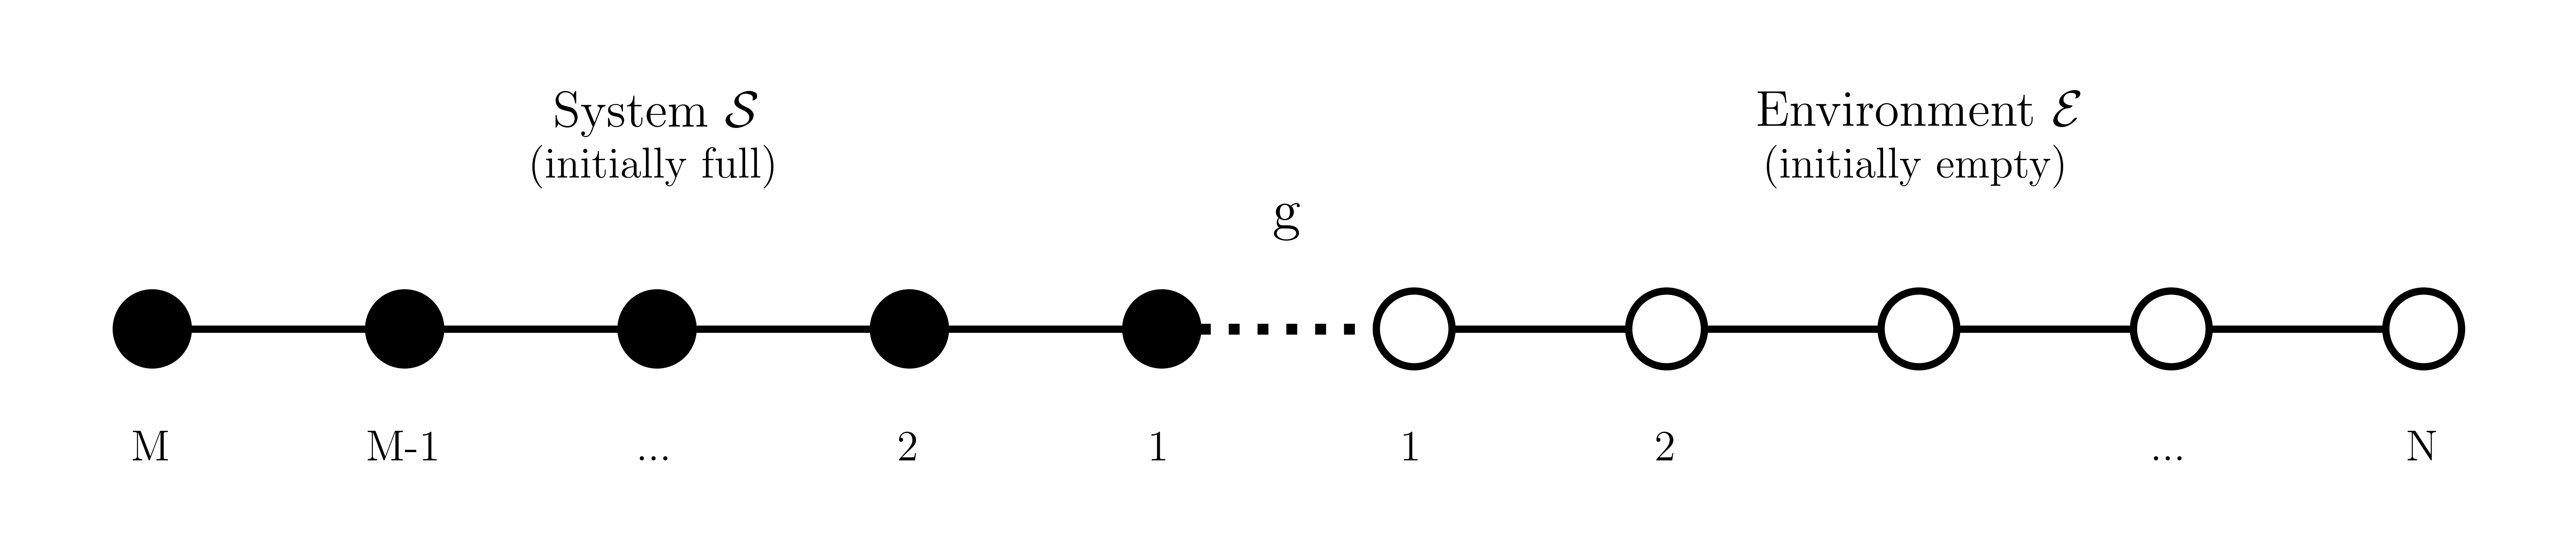
\includegraphics[width=1.0\textwidth]{figures/fermion_model_diagram.png}
    \caption{One-dimensional free-fermion chain coupled to a large environment. Filled circles denote the $M$-site system $\mathcal{S}$ (initially full), open circles the $N$-site environment $\mathcal{E}$ (initially empty), with boundary coupling~$g$.}
  \label{fig:chain_env_model}
\end{figure}
The total Hamiltonian of the model can be written as:
\beq
H = H_\mathrm{sys} + H_\mathrm{env} + H_\mathrm{c}
\label{eq:total_hamiltonian}
\eeq
\subsubsection{System Hamiltonian}
The system $\mathcal{S}$ consists of $M$ lattice sites with nearest-neighbor hopping:
\beq
H_\mathrm{sys} = -t_\mathrm{sys} \sum_{i=1}^{M-1} \left( c^\dagger_i c_{i+1} + \mathrm{h.c.} \right)
\label{eq:H_sys}
\eeq
where $c^\dagger_i$ and $c_i$ are fermionic creation and annihilation operators satisfying the canonical anticommutation relations:

\beq
\{c_i, c^\dagger_j\} = \delta_{ij}, \quad \{c_i, c_j\} = \{c^\dagger_i, c^\dagger_j\} = 0
\label{eq:anticommutation_system}
\eeq
The parameter $t_\mathrm{sys}$ sets the energy scale for particle hopping within the system.

\subsubsection{Environment Hamiltonian}

The environment $\mathcal{E}$ consists of $N$ lattice sites, also with nearest-neighbor hopping:
\beq
H_\mathrm{env} = -t_\mathrm{env} \sum_{i=1}^{N-1} \left( f^\dagger_i f_{i+1} + \mathrm{h.c.} \right)
\label{eq:H_env}
\eeq
where $f^\dagger_i$ and $f_i$ are fermionic operators for the environment sites with similar anticommutation relations:
\beq
\{f_i, f^\dagger_j\} = \delta_{ij}, \quad \{f_i, f_j\} = \{f^\dagger_i, f^\dagger_j\} = 0
\label{eq:anticommutation_environment}
\eeq
The system and environment fermionic operators anticommute:
\beq
\{c_i, f^\dagger_j\} = \{c_i, f_j\} = \{c^\dagger_i, f^\dagger_j\} = \{c^\dagger_i, f_j\} = 0
\label{eq:system_env_commutation}
\eeq

\subsubsection{System-Environment Coupling}

The system and environment are coupled through a boundary interaction:
\beq
H_\mathrm{c} = g \left( c^\dagger_1 f_1 + f^\dagger_1 c_1 \right)
\label{eq:H_coupling}
\eeq
This coupling allows particle exchange between the first site of the system and the first site of the environment. The coupling strength $g$ controls the rate of particle transfer and must satisfy $g \ll t_\mathrm{sys}, t_\mathrm{env}$ for the weak coupling approximation to be valid.


\subsubsection{Initial State}
The initial state consists of a completely filled system and an empty environment:
\beq
|\Psi(0)\rangle = \prod_{i=1}^M c^\dagger_i |\Omega\rangle
\label{eq:initial_state}
\eeq
where $|\Omega\rangle$ is the vacuum state satisfying:
\beq
c_i |\Omega\rangle = f_j |\Omega\rangle = 0 \quad \forall i,j
\label{eq:vacuum_conditions}
\eeq
This initial state can be explicitly written as:

\beq
|\Psi(0)\rangle = c^\dagger_1 c^\dagger_2 \cdots c^\dagger_M |\Omega\rangle
\label{eq:initial_state_explicit}
\eeq
\subsection{Qualitative Picture}
\label{sec:expected_entanglement_dynamics}
We are interested in the time evolution of the entanglement entropy between the system $\mathcal{S}$ and the environment $\mathcal{E}$ as 
particles tunnel from the filled system into the empty environment.
The total state at time $t$ is given by:
\beq
|\Psi(t)\rangle = e^{-iHt}|\Psi(0)\rangle
\eeq
The total Hilbert space can be decomposed as a tensor product of the system and environment Hilbert spaces:
\beq
\mathcal{H} = \mathcal{H}_\mathrm{sys} \otimes \mathcal{H}_\mathrm{env}
\label{eq:hilbert_space_decomposition}
\eeq
and we will study the entanglement entropy with respect to this decomposition. It is important to note that
the total state of the system plus environment remains pure for all times. As discussed in the previous chapter,
the von Neumann entanglement entropy is given by
\begin{equation}{\label{eq:SvN_def}}
\begin{split}
  S_{\mathrm{vN}}(t) & = -\mathrm{Tr}_{\mathcal{H}_{\mathrm{sys}}}\!\Big[\rho_{\mathrm{sys}}(t)\, \ln \rho_{\mathrm{sys}}(t)\Big] \\
                     & = -\mathrm{Tr}_{\mathcal{H}_{\mathrm{env}}}\!\Big[\rho_{\mathrm{env}}(t)\, \ln \rho_{\mathrm{env}}(t)\Big]
\end{split}
\end{equation}
where the reduced density operators are
$\rho_{\mathrm{sys}}(t) = \mathrm{Tr}_{\mathcal{H}_{\mathrm{env}}}|\Psi(t)\rangle\langle\Psi(t)|$ and
$\rho_{\mathrm{env}}(t) = \mathrm{Tr}_{\mathcal{H}_{\mathrm{sys}}}|\Psi(t)\rangle\langle\Psi(t)|$.
The calculation in this thesis focuses on $\rho_{\mathrm{sys}}$, for which one has the following argument
for why Page-curve-like behavior is expected.
The initial particle imbalance between system $\mathcal{S}$ and environment $\mathcal{E}$ will lead to decay of the number of particles in the system.
\begin{equation}
  m(t) = \bra{\Psi(t)}\left(\sum_{i=1}^{M} c_i^\dagger c_i\right) \ket{\Psi(t)}
\end{equation}

Initially, $m(0)= M$ and after a short transient period, one expects an approximately constant discharge current
\(I(t)\equiv -\dot m(t)\), which can be interpreted as particle-hole pair production at the boundary between system and environment.
The holes travel into the system $\mathcal{S}$ and the particles into the environment $\mathcal{E}$.
Semiclassically, particle current and entanglement generation are proportional to one another.
This leads to linear entanglement growth, with a proportionality factor set by the particle current $I$.
At late times the particles will be spread out approximately evenly throughout system $\mathcal{S}$ and environment $\mathcal{E}$. 
Since there are $M$ particles distributed uniformly over $M+N$ sites, the probability of finding a particle at any given site is $M/(M+N)$.
The expected number of particles in the $M$-site system is therefore
\begin{equation}\label{eq:long_time_m}
  \lim_{t\to \infty} m(t) = M \times \frac{M}{M+N} = \frac{M^2}{M+N}
\end{equation}
which is small for sufficiently large environments. Notice that strictly speaking the long time limit in \eqref{eq:long_time_m} requires 
additional averaging over a suitable time window in order to suppress
fluctuations, but this detail plays no role in the following analysis.
For $N\gg M^2$, the late-time occupation of $\mathcal{S}$ is parametrically small, so asymptotically the state approaches product form:
\begin{equation}
  \ket{\psi(t)} \approx \ket{\Omega}_\mathrm{sys} \otimes \ket{\Phi}_\mathrm{env}
\end{equation}
and therefore vanishing entanglement up to finite-size recurrences.

\paragraph{Effective Hilbert Space Argument.}
A more complete picture can be deduced from the observation that at any given time one can approximately replace 
$\mathcal{H}_\mathrm{sys}$ with an effective Hilbert space $\mathcal{H}_\mathrm{sys}^{(\mathrm{eff})}$ for $m(t)$ 
spinless fermions on $M$ lattice sites with dimension:
\begin{equation}
  \dim \mathcal{H}_\mathrm{sys}^{(\mathrm{eff})} = \binom{M}{m(t)}
\end{equation}
Since the entanglement entropy is bounded by the logarithm of the Hilbert space dimension, this approximation leads to:
\begin{equation}
  S_{\mathrm{vN}}(t) \leq \ln \dim \mathcal{H}_\mathrm{sys}^{(\mathrm{eff})}
\end{equation}
Using the Stirling approximation $\ln n! \approx n \ln n - n$ for the binomial coefficient, we obtain:
\begin{equation}\label{eq:Sent_Heff}
  S_{\mathrm{vN}}(t) \lesssim m(t) \ln\left(\frac{M}{m(t)}\right) + \bigl(M - m(t)\bigr) \ln\left(\frac{M}{M - m(t)}\right)
\end{equation}
This expression trivially reproduces both the short and long time limits: at $t=0$ when $m(0)=M$, the bound 
gives $S_{\mathrm{vN}}=0$; at late times when $m(t)\to 0$, it again gives $S_{\mathrm{vN}}\to 0$. Crucially, the 
bound is maximized when the system is half-full, i.e., when $m(t) = M/2$, consistent with the Page curve 
reaching its maximum at the Page time.

It is important to note that this argument based on replacing $\mathcal{H}_\mathrm{sys}$ with 
$\mathcal{H}_\mathrm{sys}^{(\mathrm{eff})}$ is not rigorous since it neglects fluctuations around the 
expectation value of the number of particles in the system $m(t)$. However, for our model we can
calculate the entanglement entropy exactly and confirm this intuitive picture.

Page curve entanglement dynamics should therefore be expected for this model.
\section{Numerical Solution}
There are many well-established numerical procedures for calculating entanglement entropy in 1D systems. We will use
Peschel's~\cite{Peschel_2003} correlation-matrix formalism to obtain the entanglement entropy of the subsystem.
Our goal is to calculate the reduced density matrix of the subsystem $\rho_{\mathrm{sys}}$ and then extract the relevant entanglement measures.
The key insight is that for quadratic (free) fermion Hamiltonians, the time evolution remains within the manifold of Gaussian states. 
Gaussian states have the remarkable property that all many-body observables can be computed from two-point correlation functions via 
Wick's theorem. This dramatically simplifies the calculation: instead of tracking an exponentially large many-body density matrix 
(which would have dimension $2^M \times 2^M$ for $M$ sites), we need only compute and diagonalize the $M \times M$ correlation matrix 
of the subsystem. This reduces the computational complexity from exponential to polynomial scaling, making the problem tractable even 
for relatively large systems.

\subsection{The Peschel Formalism}
\label{sec:peschel_formalism}
We now show why, in quadratic (free) fermion problems, the reduced density matrix of a spatial subsystem is 
completely determined by the two-point correlator restricted to that subsystem, and how to compute entanglement quantities directly from it. 
Our presentation closely follows the classic results of Peschel~\cite{Peschel_2003}.

For any Gaussian state (ground state or time-evolved under a quadratic Hamiltonian), Wick’s theorem holds. Consequently, all higher-order 
correlators on a subset of sites \(\mathcal{S}\) are functions of the two-point correlator on \(\mathcal{S}\):
\beq
 C_{mn}(t)=\avg{c_m^\dagger(t) c_n(t)}\,, \qquad m,n\in\mathcal{S}.
 \label{eq:subC_def}
\eeq
Here, $C_{mn}(t)$ is the correlation matrix with elements representing the expectation value of creating a particle at site $m$ and 
annihilating one at site $n$ at time $t$. For $m=n$, this gives the occupation number of site $m$; for $m \neq n$, it captures quantum coherence between sites. 
To understand why this matrix suffices, recall that Wick's theorem states that for a Gaussian state, any higher-order expectation value factors 
into products of two-point functions. For instance, the four-point function satisfies
\beq
\avg{c_i^\dagger c_j^\dagger c_k c_\ell} = \avg{c_i^\dagger c_\ell}\avg{c_j^\dagger c_k} 
- \avg{c_i^\dagger c_k}\avg{c_j^\dagger c_\ell} + \avg{c_i^\dagger c_j^\dagger}\avg{c_k c_\ell}.
\label{eq:wick_example}
\eeq
Note that for states with fixed particle number (such as our initial state), the anomalous terms $\avg{c_i^\dagger c_j^\dagger}$ and $\avg{c_k c_\ell}$ vanish, simplifying the expression to only the first two terms.
Since our Hamiltonian is quadratic and preserves the Gaussian property under time evolution, $C_{\mathcal{S}}(t)$ contains all information 
about the subsystem state at any time $t$. This matrix completely characterizes the quantum state of the subsystem.
The reduced density matrix \(\rho_{\mathcal{S}}(t)\) must be Gaussian because tracing over environment degrees of freedom preserves the Gaussian structure---both system and environment evolve under quadratic Hamiltonians, and the partial trace operation cannot introduce non-Gaussian features. Any Gaussian density operator can be written in the thermal-like form (exponential in a quadratic form):
\beq
 \rho_{\mathcal{S}}(t)=\mathcal{K}\,\exp\!\Big(-\sum_{i,j\in\mathcal{S}} H_{ij}(t)\, c_i^\dagger c_j\Big),
 \label{eq:rho_gaussian}
\eeq
for some Hermitian kernel \(H(t)\) (called the entanglement or modular Hamiltonian) and a normalization constant \(\mathcal{K}\). 
This form ensures that the state remains within the class of Gaussian states, which are fully determined by their two-point correlators. The key advantage is computational: instead of tracking an exponentially large many-body density matrix (dimension $2^M \times 2^M$ for $M$ sites), we need only compute the $M \times M$ correlation matrix.

\paragraph{Evolving the full correlator and restricting to \(\mathcal{S}\).}
Write the single-particle tight-binding matrix corresponding to \(H\) in Eq.~\eqref{eq:total_hamiltonian} as \(h\) in the site basis ordered as \((\mathcal{S},\mathcal{E})\). This means we construct an $(M+N) \times (M+N)$ matrix where the first $M$ rows and columns correspond to system sites and the last $N$ rows and columns correspond to environment sites. The one-body propagator is
\beq
 U(t)=e^{-i h t}\,.
 \label{eq:U_t}
\eeq
Because the full Hamiltonian is quadratic, the many-body time evolution reduces to single-particle evolution. Equal-time correlators evolve unitarily:
\beq
 \hat C(t)=U(t)\, \hat C(0)\, U^\dagger(t)\,,
 \label{eq:C_full_evolve}
\eeq
where \(\hat C\) denotes the correlator on all \(M{+}N\) sites. For our initial condition in Eq.~\eqref{eq:initial_state} (system full, environment empty),
\beq
 \hat C(0)=
 \begin{pmatrix}
 \mathbb{I}_M & 0\\
 0 & 0_N
 \end{pmatrix}.
 \label{eq:C0_block}
\eeq
The subsystem correlator is obtained by restriction to the principal \(M\times M\) block:
\beq
 C_{\mathcal{S}}(t)=\big[\hat C(t)\big]_{1:M,\,1:M}.
 \label{eq:restrict}
\eeq
This restriction is equivalent to tracing out the environment degrees of freedom; because the coupling and time evolution are local, the full correlator evolves as a simple matrix product, and the subsystem information is contained in the upper-left block.

\paragraph{From \(C_{\mathcal{S}}\) to the entanglement Hamiltonian.}
Let \(\{\nu_k(t)\}\) be the eigenvalues of \(C_{\mathcal{S}}(t)\). These eigenvalues must lie in \([0,1]\) due to the fermionic occupation constraint (each mode can be either empty or occupied). In the basis that diagonalizes \(H(t)\), the modes are independent with Fermi occupancies \(\nu_k(t)=1/(e^{\varepsilon_k(t)}+1)\), which is the familiar Fermi-Dirac distribution. Inverting this relation yields the entanglement spectrum:
\beq
 \varepsilon_k(t)=\ln\!\frac{1-\nu_k(t)}{\nu_k(t)}\,.
 \label{eq:eps_from_nu}
\eeq
Promoting this eigenvalue map to a matrix identity gives Peschel’s formula
\beq
 H(t)=\ln\!\Big[(\mathbb{I}-C_{\mathcal{S}}(t))\, C_{\mathcal{S}}^{-1}(t)\Big].
 \label{eq:peschel_H}
\eeq
This matrix equation follows from the functional calculus for Hermitian matrices: if $C_{\mathcal{S}}$ and $H$ can be simultaneously diagonalized (which they can, since both are Hermitian), then the functional relation $\varepsilon = \ln[(1-\nu)/\nu]$ between their eigenvalues extends to the matrix functional relation. In other words, if $C_{\mathcal{S}} = V \,\mathrm{diag}(\nu_k)\, V^\dagger$, then $f(C_{\mathcal{S}}) = V\, \mathrm{diag}(f(\nu_k))\, V^\dagger$ for any function $f$. Thus diagonalizing \(C_{\mathcal{S}}(t)\) immediately yields the single-particle entanglement spectrum \(\{\varepsilon_k(t)\}\) and, if desired, \(H(t)\) in the site basis.

\paragraph{Entanglement entropies directly from \(C_{\mathcal{S}}\).}
All standard entanglement measures between \(\mathcal{S}\) and \(\mathcal{E}\) can be computed from \(\{\nu_k(t)\}\). In matrix form, the von Neumann entropy is
\beq
 S_{\mathrm{vN}}(t)= -\mathrm{Tr}\!\Big[C_{\mathcal{S}}\ln C_{\mathcal{S}} + (\mathbb{I}-C_{\mathcal{S}})\ln(\mathbb{I}-C_{\mathcal{S}})\Big].
 \label{eq:SvN_matrix}
\eeq
Diagonalizing $C_{\mathcal{S}}$ with eigenvalues $\nu_k$, this reduces to the simpler form
\beq
 S_{\mathrm{vN}}(t) = -\sum_k\!\Big[\nu_k\ln\nu_k + (1-\nu_k)\ln(1-\nu_k)\Big],
 \label{eq:SvN_eigenvalues}
\eeq
which is computationally more efficient. The R\'enyi entropies are
\beq
 S_\alpha(t)=\frac{1}{1-\alpha}\sum_k \ln\!\Big(\nu_k^\alpha + (1-\nu_k)^\alpha\Big)\,,\qquad \alpha>0,\ \alpha\neq 1.
 \label{eq:SRenyi_from_C}
\eeq

\paragraph{Computational procedure.}
\begin{enumerate}
  \item Build the single-particle matrix \(h\) for \(H_\mathrm{sys}{+}H_\mathrm{env}{+}H_c\) on the site basis ordered as \((\mathcal{S},\mathcal{E})\).
  \item Diagonalize once: \(h=V D V^\dagger\) with \(D=\mathrm{diag}(E_\mu)\); then \(U(t)=V e^{-i D t} V^\dagger\).
  \item Form \(\hat C(0)\) as in Eq.~\eqref{eq:C0_block} and evolve to \(\hat C(t)\) via Eq.~\eqref{eq:C_full_evolve}.
  \item Restrict to \(\mathcal{S}\): extract \(C_{\mathcal{S}}(t)\) using Eq.~\eqref{eq:restrict} and diagonalize it to get \(\{\nu_k(t)\}\).
  \item Compute \(S_{\mathrm{vN}}(t)\) and \(S_\alpha(t)\) from Eqs.~\eqref{eq:SvN_eigenvalues}–\eqref{eq:SRenyi_from_C}. If needed, recover \(H(t)\) via Eq.~\eqref{eq:peschel_H}.
\end{enumerate}

\paragraph{Example: Two-site system coupled to one-site environment.}
To illustrate the method concretely, consider the simplest nontrivial case: $M=2$ (system) and $N=1$ (environment), 
with $t_{\mathrm{sys}}=t_{\mathrm{env}}=1$ and small coupling $g=0.1$.

First, we build the Hamiltonian matrix. The single-particle Hamiltonian matrix in the site basis $(c_1, c_2, f_1)$ is:
\beq
h = \begin{pmatrix}
0 & -t_{\mathrm{sys}} & g \\
-t_{\mathrm{sys}} & 0 & 0 \\
g & 0 & 0
\end{pmatrix}
= \begin{pmatrix}
0 & -1 & 0.1 \\
-1 & 0 & 0 \\
0.1 & 0 & 0
\end{pmatrix}.
\label{eq:example_h}
\eeq
Here, site indices are ordered as (system site 1, system site 2, environment site 1). 
The upper-left $2\times 2$ block contains the system with nearest-neighbor hopping $-t_{\mathrm{sys}}$ 
between sites 1 and 2. Elements $(1,3)$ and $(3,1)$ are the coupling $+g$ between the first system site 
and the first environment site, consistent with Eq.~\eqref{eq:H_coupling}. Element $(3,3)$ corresponds 
to the single environment site with no on-site energy.

Next, we diagonalize the Hamiltonian matrix to find energy eigenstates. Numerically diagonalizing $h$ gives eigenvalues $E_\mu$ and eigenvectors forming the columns of $V$. Then:
\beq
U(t) = V\, e^{-i D t}\, V^\dagger, \quad D = \mathrm{diag}(E_1, E_2, E_3).
\label{eq:example_U}
\eeq

We then initialize and evolve the correlation matrix. The initial correlation matrix (system full, environment empty) is:
\beq
\hat C(0) = \begin{pmatrix}
1 & 0 & 0 \\
0 & 1 & 0 \\
0 & 0 & 0
\end{pmatrix}.
\label{eq:example_C0}
\eeq
At time $t$:
\beq
\hat C(t) = U(t)\, \hat C(0)\, U^\dagger(t).
\label{eq:example_Ct}
\eeq

Subsequently, we extract the subsystem correlator and diagonalize it. Restricting to the $2\times 2$ system block:
\beq
C_{\mathcal{S}}(t) = \begin{pmatrix}
\hat C_{11}(t) & \hat C_{12}(t) \\
\hat C_{21}(t) & \hat C_{22}(t)
\end{pmatrix}.
\label{eq:example_Csys}
\eeq
Diagonalizing this matrix yields eigenvalues $\nu_1(t)$ and $\nu_2(t)$ (both in $[0,1]$).

Finally, we compute the entanglement entropy. The von Neumann entropy is:
\begin{align}
S_{\mathrm{vN}}(t) &= -\Big[\nu_1(t)\ln\nu_1(t) + (1-\nu_1(t))\ln(1-\nu_1(t))\Big] \nonumber\\
&\quad -\Big[\nu_2(t)\ln\nu_2(t) + (1-\nu_2(t))\ln(1-\nu_2(t))\Big].
\label{eq:example_entropy}
\end{align}

\section{Analytical solution}
\label{sec:analytical_solution}
Since our Hamiltonian is quadratic, it allows for an analytical solution in the weak coupling 
limit $g \ll t_{\rm sys}, t_{\rm env}$. The key insight is that the many-body problem 
factorizes into $M$ independent single-particle problems, each described by a resonant level model (RLM).
In this section we first diagonalize the system Hamiltonian, then recast the coupling in the momentum basis, and finally demonstrate that in the weak-coupling regime the dynamics factorize into independent resonant level models with universal entanglement dynamics.
\subsection{Diagonalization of System Hamiltonian}
\label{subsec:diagonalization}
\begin{equation}
H_{\text{sys}} = -t_{\text{sys}} \sum_{i=1}^{M-1} \left(c_i^\dagger c_{i+1} + c_{i+1}^\dagger c_i\right)
\label{eq:system_hamiltonian}
\end{equation}
We now diagonalize $H_{\text{sys}}$ to find eigenvalues $\omega_k$ and eigenvectors $|\psi_k\rangle$:
\begin{align}
H_{\text{sys}} |\psi_k\rangle = \omega_k |\psi_k\rangle \label{eq:eigenvalue_problem}
\end{align}
Let $|\psi_k\rangle = \sum_{i=1}^M \psi_k(i) |i\rangle$ where $|i\rangle$ represents a state with a single particle at site $i$.
Acting with $H_{\text{sys}}$ on $|\psi_k\rangle$:
\begin{align}
H_{\text{sys}} |\psi_k\rangle &= -t_{\text{sys}} \sum_{i=1}^{M-1} \left( c_i^\dagger c_{i+1} + c_{i+1}^\dagger c_i \right) \sum_{j=1}^M \psi_k(j) |j\rangle \nonumber\\
&= -t_{\text{sys}} \sum_{i=1}^{M-1} \sum_{j=1}^M \psi_k(j) \left( \delta_{i,j} |i+1\rangle + \delta_{i+1,j} |i\rangle \right) \nonumber\\
&= -t_{\text{sys}} \sum_{i=1}^M \left[ \psi_k(i-1) + \psi_k(i+1) \right] |i\rangle \label{eq:H_action}
\end{align}
where we define $\psi_k(0) = \psi_k(M+1) = 0$ (open boundary conditions).
From the eigenvalue equation \eqref{eq:eigenvalue_problem} and \eqref{eq:H_action}:
\begin{align}
-t_{\text{sys}} \sum_{i=1}^M \left[ \psi_k(i-1) + \psi_k(i+1) \right] |i\rangle = \omega_k \sum_{i=1}^M \psi_k(i) |i\rangle
\end{align}
Comparing coefficients of $|i\rangle$:
\begin{align}
-t_{\text{sys}} \left[ \psi_k(i-1) + \psi_k(i+1) \right] = \omega_k \psi_k(i) \label{eq:discrete_schrodinger}
\end{align}
This is the discrete Schrödinger equation for a tight-binding chain.
We consider a sine-wave ansatz consistent with the boundary conditions $\psi_k(0) = \psi_k(M+1) = 0$:
\begin{align}
\psi_k(i) = A \sin\left(\frac{\pi k i}{M+1}\right), \quad k = 1, 2, \ldots, M \label{eq:sine_ansatz}
\end{align}
Verify boundary conditions:
\begin{align}
\psi_k(0) &= A \sin(0) = 0 \quad  \\
\psi_k(M+1) &= A \sin(\pi k) = 0 \quad 
\end{align}
Substituting \eqref{eq:sine_ansatz} into \eqref{eq:discrete_schrodinger}:
\begin{align}
&-t_{\text{sys}} \left[ A \sin\left(\frac{\pi k (i-1)}{M+1}\right) + A \sin\left(\frac{\pi k (i+1)}{M+1}\right) \right] \nonumber\\
&\quad = \omega_k A \sin\left(\frac{\pi k i}{M+1}\right)
\end{align}
Using the trigonometric identity  
\[
\sin(X - Y) + \sin(X + Y) = 2 \sin(X) \cos(Y),
\]  
with $X = \frac{\pi k i}{M + 1}$ and $Y = \frac{\pi k}{M + 1}$, we obtain:
\begin{align}
\sin\left(\frac{\pi k (i-1)}{M+1}\right) + \sin\left(\frac{\pi k (i+1)}{M+1}\right) &= 2\sin\left(\frac{\pi k i}{M+1}\right)\cos\left(\frac{\pi k}{M+1}\right)
\end{align}
Substituting this back into the equation:
\begin{align}
-t_{\text{sys}} \cdot 2A\sin\left(\frac{\pi k i}{M+1}\right)\cos\left(\frac{\pi k}{M+1}\right) = \omega_k A \sin\left(\frac{\pi k i}{M+1}\right)
\end{align}
Canceling common factors:
\begin{align}
\omega_k = -2t_{\text{sys}} \cos\left(\frac{\pi k}{M+1}\right) \label{eq:eigenvalues_detailed}
\end{align}
\textbf{Normalization and Orthogonality.}
We require $\langle \psi_k | \psi_k \rangle = 1$:
\begin{align}
\sum_{i=1}^M |\psi_k(i)|^2 &= \sum_{i=1}^M A^2 \sin^2\left(\frac{\pi k i}{M+1}\right) = 1
\end{align}
Using the identity (shown in Appendix~\ref{app:sine_identity})
\begin{equation}
\sum_{i=1}^M \sin^2\left(\frac{\pi k i}{M+1}\right) = \frac{M+1}{2} \quad \text{for integer } k \in \{1, 2, \ldots, M\},
\end{equation}
we obtain:
\begin{align}
A^2 \cdot \frac{M+1}{2} = 1 \implies A = \sqrt{\frac{2}{M+1}}
\end{align}
Normalized eigenfunctions:
\begin{align}
\psi_k(i) = \sqrt{\frac{2}{M+1}} \sin\left(\frac{\pi k i}{M+1}\right) \label{eq:normalized_eigenfunctions}
\end{align}
Orthogonality verification:
For $k \neq k'$:
\begin{align}
\langle \psi_k | \psi_{k'} \rangle &= \sum_{i=1}^M \psi_k^*(i) \psi_{k'}(i) \nonumber\\
&= \frac{2}{M+1} \sum_{i=1}^M \sin\left(\frac{\pi k i}{M+1}\right) \sin\left(\frac{\pi k' i}{M+1}\right) = 0
\end{align}
This follows from the orthogonality of sine functions on the discrete grid.
\subsection{Transformation to Diagonal Basis}
We introduce new creation and annihilation operators for the momentum basis:
\begin{align}
c_k^\dagger &= \sum_{i=1}^M \psi_k(i) c_i^\dagger = \sum_{i=1}^M \sqrt{\frac{2}{M+1}} \sin\left(\frac{\pi k i}{M+1}\right) c_i^\dagger \label{eq:ck_definition}\\
c_k &= \sum_{i=1}^M \psi_k^*(i) c_i = \sum_{i=1}^M \sqrt{\frac{2}{M+1}} \sin\left(\frac{\pi k i}{M+1}\right) c_i \label{eq:ck_annihilation}
\end{align}

\paragraph{Initial state in momentum basis.}
The initial state in the site basis is $|\Psi(0)\rangle = \prod_{i=1}^M c_i^\dagger |\Omega\rangle$, corresponding to all sites occupied. In the momentum basis, this transforms to:
\begin{equation}
|\Psi(0)\rangle = \prod_{k=1}^M c_k^\dagger |\Omega\rangle
\end{equation}
This can be verified by noting that the unitary transformation preserves fermion number: the state has exactly $M$ 
particles in both representations. Each momentum mode $k$ starts with occupation $n_k(0) = \langle c_k^\dagger c_k \rangle = 1$, 
confirming that all momentum modes are initially filled.
Using the single-particle matrix representation, one can write
\begin{align}
H_{\text{sys}} &= \sum_{k,l=1}^M c_k^\dagger c_l \sum_{i,j=1}^M \psi_k(i)\, h_{ij}\, \psi_l(j),
\end{align}
where \(h_{ij}=-t_{\mathrm{sys}}(\delta_{i,j+1}+\delta_{i,j-1})\).
Using trigonometric identities and orthogonality relations, this simplifies to:
\begin{equation}
H_{\text{sys}} = \sum_{k=1}^M \omega_k c_k^\dagger c_k
\end{equation}
with $\omega_k = -2 t_{\text{sys}} \cos\left(\frac{\pi k}{M+1}\right)$.

\paragraph{Coupling term in momentum basis.}
Using the inverse transformation for $c_1$:
\begin{equation}
c_1 = \sum_{k=1}^M \sqrt{\frac{2}{M+1}} \sin\left(\frac{\pi k \cdot 1}{M+1}\right) c_k = \sum_{k=1}^M \sqrt{\frac{2}{M+1}} \sin\left(\frac{\pi k}{M+1}\right) c_k
\end{equation}
Therefore:
\begin{equation}
c_1^\dagger = \sum_{k=1}^M \sqrt{\frac{2}{M+1}} \sin\left(\frac{\pi k}{M+1}\right) c_k^\dagger
\end{equation}
Substituting into the coupling term:
\begin{align}
H_c &= g\left(\left[\sum_{k=1}^M \sqrt{\tfrac{2}{M+1}} \sin\left(\tfrac{\pi k}{M+1}\right) c_k^\dagger\right] f_1\right) \\
&\quad +\; g\left(f_1^\dagger \left[\sum_{k=1}^M \sqrt{\tfrac{2}{M+1}} \sin\left(\tfrac{\pi k}{M+1}\right) c_k\right]\right) \\
&= g \sum_{k=1}^M \sqrt{\tfrac{2}{M+1}} \sin\left(\tfrac{\pi k}{M+1}\right) \left(c_k^\dagger f_1 + f_1^\dagger c_k\right)
\end{align}
Defining the hybridization matrix elements:
\begin{equation}
V_k = g\sqrt{\frac{2}{M+1}} \sin\left(\frac{\pi k}{M+1}\right)
\end{equation}
We obtain:
\begin{equation}
H_c = \sum_{k=1}^M V_k \left(c_k^\dagger f_1 + f_1^\dagger c_k\right)
\end{equation}
This leads to an equivalent description in terms of single particle levels $ c_k^\dagger,c_k$.
The complete Hamiltonian in momentum basis is:
\begin{equation}
H = \sum_{k=1}^M \omega_k c_k^\dagger c_k + \sum_{k=1}^M V_k \left(c_k^\dagger f_1 + f_1^\dagger c_k\right) + H_{\text{env}}.
\label{eq:H_total_momentum}
\end{equation}
This transformation reveals the system as a collection of $M$ single-particle levels with energies $\omega_k$, 
each coupled to the environment boundary with strength $V_k$. The next step is understanding how these couplings induce decay.

\subsection{Boundary Coupling and Hybridization}
\label{subsec:boundary_dos}

To understand when the momentum modes $k$ can be treated independently, we must first characterize 
how each couples to the environment. The coupling occurs exclusively through the boundary site $f_1$ [Eq.~\eqref{eq:H_coupling}], 
so the relevant spectral quantity is the \emph{local} (surface) density of states at that boundary site, not the bulk DOS. This distinction is crucial: boundary coupling probes only states with amplitude at the surface.

To understand the decay process physically, we must consider the \emph{Density of States} (DOS), $\rho(E)$, which essentially counts the number of available energy levels in the environment per unit energy interval. It can be thought of as the "capacity" of the environment to accept particles at a specific energy $E$.
However, our system does not couple to the entire environment at once; it connects only at a single boundary point. Therefore, what matters is not just how many states exist, but how many of them have a non-zero wavefunction amplitude at the contact point. This is captured by the \emph{Local Density of States} (LDOS), $\rho_{\mathrm{loc}}(E)$. If the environment has many states at energy $E$, but all of them have nodes (zero amplitude) at the boundary, the system cannot decay into them.

When a discrete quantum level from our system couples to this continuum of environment states, it undergoes \emph{hybridization}. The discrete state mixes with the continuum states, causing it to lose its sharp energy definition. It acquires a finite energy width, denoted by $\Gamma$. This width $\Gamma$ is directly related to the decay rate: a broader resonance implies a faster leakage of particles into the environment.
Formally, when a discrete level is coupled to a continuum, its decay rate is proportional to the local DOS at the level energy. In our case, only those environment eigenstates that have nonzero amplitude at the boundary site $f_1$ can participate in the decay. Therefore, the relevant quantity is not the bulk DOS of the infinite chain, but the \emph{local} (or surface) DOS at site 1, denoted $\rho_{\mathrm{loc}}(E)$.

\subsubsection{Surface Green's function and local density of states}

The local DOS at the boundary is most conveniently obtained from the \emph{retarded Green's function}
of a semi-infinite tight-binding chain with hopping $t_{\mathrm{env}}$. The retarded Green's function
$g^R_{11}(E)$ is defined as the matrix element of $(E + i0^+ - H_{\mathrm{env}})^{-1}$ at the boundary site.
Its imaginary part encodes how strongly states of energy $E$ are present at that site, and the standard
relation
\begin{equation}
 \rho_{\mathrm{loc}}(E) = -\frac{1}{\pi}\,\mathrm{Im}\, g^{R}_{11}(E)
\end{equation}
connects the two. This is why we first compute $g^{R}_{11}(E)$ and then extract $\rho_{\mathrm{loc}}(E)$ from it.

For a semi-infinite tight-binding chain, the surface Green's function takes the form
\begin{equation}
 g^{R}_{11}(E) = \frac{E - i\sqrt{4 t_{\mathrm{env}}^2 - E^2}}{2 t_{\mathrm{env}}^2}\,, \qquad |E|<2 t_{\mathrm{env}}.
 \label{eq:surface_GF}
\end{equation}
This explicit expression can be derived using a simple self-consistency argument based on the self-similarity of the semi-infinite chain. If we remove the first site, the remaining chain (starting from site 2) is identical to the original one. Therefore, the Green's function at site 2 (in the presence of the rest of the chain) is identical to $g^{R}_{11}(E)$.
The effect of the rest of the chain on site 1 can be viewed as a self-energy term $\Sigma_{\mathrm{chain}} = |t_{\mathrm{env}}|^2 g^{R}_{11}(E)$, describing a process where a particle hops to site 2, propagates through the semi-infinite chain, and hops back.
This leads to the Dyson equation:
\begin{equation}
 g^{R}_{11}(E) = \frac{1}{E + i0^+ - t_{\mathrm{env}}^2 \, g^{R}_{11}(E)}\,,
\end{equation}
which is a quadratic equation for $g^{R}_{11}(E)$. Solving this equation and choosing the branch
with $\Im g^{R}_{11}(E) < 0$ (retarded boundary condition) leads directly to Eq.~\eqref{eq:surface_GF}.
The corresponding \emph{local} density of states at the boundary is then
\begin{equation}
 \rho_{\mathrm{loc}}(E) = -\frac{1}{\pi}\,\mathrm{Im}\, g^{R}_{11}(E)
 = \frac{1}{2\pi}\,\frac{\sqrt{4 t_{\mathrm{env}}^2 - E^2}}{t_{\mathrm{env}}^2}\,.
 \label{eq:rho_loc}
\end{equation}

When the system mode $k$ couples to the environment, its dynamics are modified by the environment's presence. In the Green's function formalism, this effect is captured by the \emph{self-energy} $\Sigma_k^{R}(E)$. To second order in the coupling $V_k$, this is given by:
\begin{equation}
 \Sigma_k^{R}(E) = |V_k|^2\, g^{R}_{11}(E)
 \label{eq:self_energy_def}
\end{equation}
with decay width
\begin{equation}
 \Gamma_k(E) = -2\,\mathrm{Im}\,\Sigma_k^{R}(E) = 2\pi\, \rho_{\mathrm{loc}}(E)\, |V_k|^2\,.
 \label{eq:Gamma_from_rho_loc}
\end{equation}
This recovers the standard Fermi's golden rule result: the decay rate of level $k$ into the continuum
is proportional to the square of the coupling $|V_k|^2$ and to the local DOS of available final
states at energy $E$.

\paragraph{Wide-band approximation (around $E\simeq 0$).}
Near the band center ($E=0$), the surface DOS is approximately constant,
\begin{equation}
 \rho_{\mathrm{loc}}(E) \approx \rho_{\mathrm{loc}}(0) = \frac{1}{\pi t_{\mathrm{env}}}\,.
 \label{eq:rho_loc_0}
\end{equation}
Hence the width becomes
\begin{equation}
 \Gamma_k \approx 2\,\frac{|V_k|^2}{t_{\mathrm{env}}}\,.
 \label{eq:Gamma_wide_band}
\end{equation}
This boundary (surface) prescription replaces bulk-DOS formulas and is the appropriate choice for end-site coupling.

\paragraph{Born–Markov assumptions.}
The validity of our analytical solution relies on two standard approximations in open quantum systems:
\begin{itemize}
    \item \textbf{Born approximation (Weak coupling):} We assume $g \ll t_{\mathrm{sys}}, t_{\mathrm{env}}$. This justifies treating the coupling perturbatively.
    \item \textbf{Markov approximation (Wide-band limit):} We assume the local DOS is slowly varying over the relevant energy scale of the system. This implies that memory effects are negligible for times $t \gtrsim 1/t_{\mathrm{env}}$.
\end{itemize}
In the Green's function language, these approximations correspond to taking the self-energy $\Sigma_k^{R}(E)$ to be constant in energy, $\Sigma_k^{R}(E) \approx \Sigma_k^{R}(\omega_k) \approx -i\Gamma_k/2$ (neglecting the small real part, or Lamb shift).
Having established that each mode $k$ acquires a width $\Gamma_k$ from coupling to the environment, we can 
now determine when these modes evolve independently.

\subsection{Resonant Level Model Factorization}
\label{subsec:rlm_factorization}
For the momentum modes to evolve independently as separate resonant level models, the key requirement is 
that their energy windows in the environment must not overlap:
\begin{equation}
    |\omega_{k+1} - \omega_k| \gg \Gamma_k(\omega_k).
\label{eq:rlm_condition}
\end{equation}
This condition ensures that the hybridization width (energy uncertainty) of each level is much smaller than 
the level spacing, so that different momentum modes $k$ couple to effectively non-overlapping spectral 
windows in the environment continuum. When this holds, dissipative cross-terms between modes become 
negligible (secular approximation).
Let us verify this condition is satisfied in the weak-coupling limit.
The energy difference between adjacent levels:
\begin{equation}
|\omega_{k+1} - \omega_k| = 2t_{\text{sys}}\left|\sin\left(\frac{\pi(2k+1)}{2(M+1)}\right)\sin\left(\frac{\pi}{2(M+1)}\right)\right|
\end{equation}
Using the identity $\cos(a) - \cos(b) = -2\sin\left(\frac{a+b}{2}\right)\sin\left(\frac{a-b}{2}\right)$:
With $a = \frac{\pi(k+1)}{M+1}$ and $b = \frac{\pi k}{M+1}$:
\begin{align}
\cos\left(\frac{\pi(k+1)}{M+1}\right) - \cos\left(\frac{\pi k}{M+1}\right) &= -2\sin\left(\frac{\pi(2k+1)}{2(M+1)}\right)\sin\left(\frac{\pi}{2(M+1)}\right)
\end{align}
Therefore:
\begin{equation}
|\omega_{k+1} - \omega_k| = 2t_{\text{sys}}\left|\sin\left(\frac{\pi(2k+1)}{2(M+1)}\right)\sin\left(\frac{\pi}{2(M+1)}\right)\right|
\end{equation}
\paragraph{Large-$M$ approximation.}
For large $M$:
\begin{equation}
\sin\left(\frac{\pi}{2(M+1)}\right) \approx \frac{\pi}{2(M+1)}
\end{equation}
And for typical $k$ (not too close to 0 or $M$):
\begin{equation}
\sin\left(\frac{\pi(2k+1)}{2(M+1)}\right) \sim \mathcal{O}(1)
\end{equation}
Therefore, for typical modes we obtain the estimate
\begin{equation}
|\omega_{k+1} - \omega_k| \approx 2t_{\text{sys}} \cdot \mathcal{O}(1) \cdot \frac{\pi}{2(M+1)} \sim \frac{\pi t_{\text{sys}}}{M+1}.
\end{equation}
The hybridization width of mode $k$ in the wide-band limit, using the boundary DOS and Eq.~\eqref{eq:Gamma_wide_band}, is
\begin{equation}
\Gamma_k(\omega_k) = 2\pi\,\rho_{\mathrm{loc}}(\omega_k)\,|V_k|^2
\approx 2\,\frac{|V_k|^2}{t_{\text{env}}}
= \frac{4 g^2}{(M+1)\, t_{\text{env}}}\, \sin^2\!\left(\frac{\pi k}{M+1}\right).
\end{equation}
For typical $k$ (away from the band edges), the sine factor is $\mathcal{O}(1)$ so we may estimate
\begin{equation}
\Gamma_k(\omega_k) \sim \frac{g^2}{(M+1)\,t_{\text{env}}}.
\end{equation}
Both the spacing and the width therefore scale as $1/M$,
\begin{equation}
|\omega_{k+1} - \omega_k| \propto \frac{t_{\text{sys}}}{M} \gg \Gamma_k(\omega_k) \propto \frac{g^2}{M\,t_{\text{env}}}\,, \label{eq:RLM_condition}
\end{equation}
so the factorization condition reduces to a simple inequality between couplings:
\begin{equation}
g^2 \ll t_{\text{sys}}\, t_{\text{env}}\,,
\end{equation}
or equivalently
\begin{equation}
g \ll \sqrt{t_{\text{sys}} t_{\text{env}}}\,.
\label{eq:RLM_condition_conclusion}
\end{equation}

\begin{remark}[Band edge modes]
Strictly speaking, there is a small fraction $\sim g^2/(t_{\mathrm{sys}} t_{\mathrm{env}})$ of single-particle levels 
close to $k = 1$ and $k = M$ where condition~\eqref{eq:RLM_condition} does not hold. This is because the 
dispersion relation $\omega_k = -2t_{\mathrm{sys}}\cos(\pi k/(M+1))$ becomes flat near the band edges, making the 
level spacing $|\omega_{k+1} - \omega_k|$ vanishingly small. However, in the weak-coupling limit 
$g \ll \sqrt{t_{\mathrm{sys}} t_{\mathrm{env}}}$, this fraction is negligible and does not affect the universal 
behavior derived below.
\end{remark}

When condition (\ref{eq:RLM_condition}) is satisfied, different momentum modes $k$ couple to 
non-overlapping spectral windows of the environment. Although all modes physically couple through 
the same boundary site $f_1$, in the \emph{energy domain} they interact with disjoint sets of 
environment eigenstates. This effective separation in energy space—not in real space—allows us to 
treat each mode as coupling to its own independent bath.
Mathematically, the environment Hilbert space can be partitioned as a useful approximation:
\begin{equation}
\mathcal{H}_{\text{env}} = \bigoplus_{k=1}^M \mathcal{H}_{\text{env}}^{(k)}, \quad \text{where } \mathcal{H}_{\text{env}}^{(k)} = \text{span}\{|E\rangle : |E - \omega_k| \lesssim \Gamma_k\}.
\end{equation}
Because the hybridization widths $\Gamma_k$ are much smaller than level spacings $|\omega_{k+1} - \omega_k|$, these subspaces have negligible overlap, and the dynamics factorizes. This should be understood as a physical approximation: in the weak-coupling and secular limits, environment states near different $\omega_k$ contribute independently to the dynamics. This is equivalent to invoking the \emph{secular approximation}: neglecting dissipative cross-terms between modes with well-separated Bohr frequencies.

\subsubsection{Independent resonant level models}

Under this approximation, our model becomes a collection of $M$ independent resonant level models (RLMs):
\begin{equation}
H_k^{(\text{RLM})} = \omega_k c_k^\dagger c_k + \sum_i V_k \left(c_k^\dagger a_{k,i} + a_{k,i}^\dagger c_k\right) + \sum_i \varepsilon_i a_{k,i}^\dagger a_{k,i}.
\label{eq:RLM_hamiltonian}
\end{equation}
where:
\begin{itemize}
\item $\omega_k$ is the energy of level $k$
\item $c_k^\dagger, c_k$ create/annihilate particles in level $k$
\item $a_{k,i}^\dagger, a_{k,i}$ create/annihilate particles in environment mode $i$ coupled to level $k$
\item $\varepsilon_i$ are the energies of environment modes
\item $V_k$ is the coupling strength
\end{itemize}
Hybridization (decay width) for level $k$ follows directly from Eq.~\eqref{eq:Gamma_wide_band} and the definition of $V_k$,
\begin{equation}
\Gamma_k(E) = 2\,\frac{|V_k|^2}{t_{\text{env}}}
= \frac{4 g^2}{(M+1)\, t_{\text{env}}}\, \sin^2\!\left(\frac{\pi k}{M+1}\right).
\label{eq:Gamma_k}
\end{equation}
The reduced density operator of the system is then a direct product of reduced density operators of $M$ resonant level models
\begin{equation}
\rho_{\text{sys}}(t) = \bigotimes_{k=1}^M \rho_k^{(\text{RLM})}(t).
\label{eq:rho_sys_factorized}
\end{equation}
Within the secular weak-coupling approximation, the effective factorized Hamiltonian \(H_{\mathrm{eff}}=\sum_k H_k^{(\mathrm{RLM})}\) gives
\begin{equation}
e^{-iH_{\mathrm{eff}}t} = \prod_{k=1}^M e^{-iH_k^{(\text{RLM})}t}
\end{equation}
and therefore the reduced density matrix factorizes to the same level of approximation.
\paragraph{Two-level structure.}
For each resonant level model
\begin{equation}
\rho_k^{(\text{RLM})}(t) = \begin{pmatrix}
n_k(t) & 0 \\
0 & 1-n_k(t)
\end{pmatrix}.
\label{eq:rho_k_form}
\end{equation}
where $n_k(t) = \langle c_k^\dagger c_k \rangle_t$ is the occupation probability.
The key remaining question is: how do these occupation numbers evolve in time?
\subsubsection{Time evolution: exponential decay}
\label{subsec:time_evolution_derivation}

In the wide flat band limit ($t_{\mathrm{env}} \gg t_{\mathrm{sys}}$), the local density of states at the boundary is approximately constant, $\rho_{\mathrm{loc}}(E) \approx \rho_{\mathrm{loc}}(0)$. It is known that in this limit the impurity orbital occupation of a resonant level model decays purely exponentially~\cite{PhysRevB.32.4410,Langreth1991}:
\begin{equation}
n_k(t) = e^{-\Gamma_k t}
\end{equation}
where $\Gamma_k$ is the level width defined in Eq.~\eqref{eq:Gamma_k}.
This is an \emph{exact} result for the wide-band resonant level model: since the Hamiltonian~\eqref{eq:RLM_hamiltonian} is quadratic and the bath density of states is taken as constant, the retarded Green's function of the impurity level is
\begin{equation}
G_k^R(t) = -i\,\theta(t)\,e^{-i\omega_k t}\,e^{-\Gamma_k t/2},
\end{equation}
and with the bath initially in the vacuum state the occupation follows as $n_k(t) = |G_k^R(t)|^2 = e^{-\Gamma_k t}$.
Physically, particles tunnel irreversibly from system level $k$ into the empty environment at rate $\Gamma_k$.

This exponential decay is valid for times much shorter than the recurrence time $t_{\mathrm{rec}} \sim N/(2t_{\mathrm{env}})$ set by ballistic propagation and reflection at the far boundary of a finite environment chain.

\subsection{Mode Occupation Dynamics}

With initial condition $n_k(0) = 1$ (all system modes fully occupied) and the exponential decay law, we have
\begin{equation}
n_k(t) = e^{-\Gamma_k t}\,.
\end{equation}
In the wide-band limit around $E\simeq 0$, Eqs.~\eqref{eq:rho_loc_0} and \eqref{eq:Gamma_k} give
\begin{equation}
\Gamma_k \approx 2\,\frac{|V_k|^2}{t_{\mathrm{env}}} = 2\,\frac{g^2}{t_{\mathrm{env}}}\,\frac{2}{M+1}\, \sin^2\!\left(\frac{\pi k}{M+1}\right) = \frac{4 g^2}{(M+1) t_{\mathrm{env}}}\, \sin^2\!\left(\frac{\pi k}{M+1}\right).
\end{equation}
Therefore, the complete time evolution is
\begin{equation}
n_k(t) = \exp\!\left[-\,\frac{4 g^2}{(M+1)\, t_{\mathrm{env}}}\, \sin^2\!\left(\frac{\pi k}{M+1}\right) t\right].
\label{eq:nk_explicit}
\end{equation}

\paragraph{Physical interpretation.}
The $\sin^2(\pi k/(M+1))$ factor reflects the spatial overlap between momentum mode $k$ and the boundary coupling site. Modes with $k \approx M/2$ have maximum amplitude at the boundary and decay fastest, while modes with $k \approx 1$ or $k \approx M$ have small boundary amplitude and decay more slowly. This mode-dependent decay is the microscopic origin of the Page curve: different modes empty at different rates, creating intermediate states with maximum entanglement.

\subsubsection{Entanglement entropy from factorization}

The factorization of the reduced density matrix Eq.~\eqref{eq:rho_sys_factorized} allows us to compute the entanglement entropy as a sum over independent contributions:
\begin{align}
S^{(\text{vN})}(t) &= -\operatorname{Tr}[\rho_{\text{sys}}(t) \ln \rho_{\text{sys}}(t)]\\
&= -\operatorname{Tr}\left[\bigotimes_{k=1}^M \rho_k^{(\text{RLM})}(t) \ln \left(\bigotimes_{k=1}^M \rho_k^{(\text{RLM})}(t)\right)\right]\\
&= -\sum_{k=1}^M \operatorname{Tr}[\rho_k^{(\text{RLM})}(t) \ln \rho_k^{(\text{RLM})}(t)]\\
&= -\sum_{k=1}^M \left[n_k(t) \ln n_k(t) + (1-n_k(t)) \ln(1-n_k(t))\right]
\end{align}

This additivity relies on the secular-approximation logic: in the $\{c_k\}$ basis, dissipative cross-terms are neglected so the reduced one-body correlator is (approximately) diagonal, making the entropy a sum of binary entropies. Each mode contributes independently to the total entanglement.

With the explicit form $n_k(t)$ from Eq.~\eqref{eq:nk_explicit}, we now have a complete analytical description of the entanglement dynamics. The next step is taking the continuum limit to reveal universal behavior.

\subsection{Continuum Limit and Universal Behavior}
\label{subsec:universal_behavior}

For large system size $M \gg 1$, the discrete sum over modes can be replaced by an integral, revealing universal scaling behavior independent of microscopic details.

\subsubsection{Continuum limit}

For large $M$, we define the continuous momentum variable $q = \frac{\pi k}{M+1} \in (0,\pi)$. The spacing between consecutive $q$ values is $\Delta q = \frac{\pi}{M+1} \approx \frac{\pi}{M}$. We can thus replace discrete sums by integrals according to the rule:
\begin{equation}
\sum_{k=1}^M f\!\left(\frac{\pi k}{M+1}\right) \;\approx\; \frac{M}{\pi} \sum_{k=1}^M f(q_k) \Delta q \;\longrightarrow\; \frac{M}{\pi} \int_0^{\pi} f(q)\, dq, \qquad M\to\infty.
\end{equation}

This continuum limit transforms both observables (particle number, entanglement entropy) into integrals over the continuous momentum $q$.

\paragraph{Particle number in continuum limit.}
The total particle number becomes:
\begin{align}
m(t) &= \sum_{k=1}^M n_k(t) \to \frac{M}{\pi} \int_0^{\pi} n(q,t)\, dq,
\end{align}
or, normalizing by system size:
\begin{equation}
\frac{m(t)}{M} = \frac{1}{\pi} \int_0^{\pi} n(q,t)\, dq.
\end{equation}

\paragraph{Entanglement entropy in continuum limit.}
Similarly, the von Neumann entropy per site becomes:
\begin{equation}
\frac{S^{(\text{vN})}(t)}{M} = -\frac{1}{\pi} \int_0^{\pi} dq \, \Big[n(q,t) \ln n(q,t) + (1-n(q,t)) \ln(1-n(q,t))\Big].
\label{eq:SvN_continuum}
\end{equation}

\subsubsection{Dimensionless time and universal form}

From the exponent in Eq.~\eqref{eq:nk_explicit}, the natural time scale emerges:
\begin{equation}
t_{\text{natural}} = \frac{(M+1)\, t_{\mathrm{env}}}{4 g^2}\,.
\end{equation}

We define the dimensionless time
\begin{equation}
  	\tau = \frac{t}{t_{\text{natural}}} = \frac{4 g^2}{(M+1)\, t_{\mathrm{env}}}\, t\,,
\label{eq:tau_def}
\end{equation}
and for large $M$ we may replace $M+1 \approx M$ when converting sums to integrals.

Using $q = \pi k/(M+1)$ and the dimensionless time $\tau$, the occupation number takes the universal form:
\begin{equation}
n(q,\tau) = \exp\!\big(-\tau \, \sin^2 q\big), \qquad q\in[0,\pi].
\label{eq:nq_tau}
\end{equation}

This is the key result: the dynamics depend only on the dimensionless time $\tau$ and continuous momentum $q$, independent of the specific values of $g$, $t_{\text{sys}}$, $t_{\text{env}}$, $M$, or $N$. All systems in the appropriate parameter regime exhibit identical universal behavior.

\subsubsection{Page time calculation}
The dimensionless Page time $\tau_P$ is found by solving:
\begin{equation}
\frac{dS^{(\text{vN})}}{d\tau}\bigg|_{\tau=\tau_P} = 0
\end{equation}
The derivative can be evaluated explicitly as follows.
From Eq.~\eqref{eq:SvN_continuum}, using $\frac{d}{dn}[n\ln n + (1-n)\ln(1-n)] = \ln\left(\frac{n}{1-n}\right)$:
\begin{align}
\frac{dS^{(\text{vN})}}{d\tau} &= -\frac{1}{\pi} \int_0^{\pi} dq \, \ln\left(\frac{n(q,\tau)}{1-n(q,\tau)}\right) \frac{\partial n(q,\tau)}{\partial\tau}
\end{align}
With $n(q,\tau) = e^{-\tau \sin^2 q}$:
\begin{equation}
\frac{\partial n(q,\tau)}{\partial\tau} = -\sin^2 q\, e^{-\tau \sin^2 q} = -\sin^2 q\, n(q,\tau)
\end{equation}
Therefore:
\begin{align}
\frac{dS^{(\text{vN})}}{d\tau} &= \frac{1}{\pi} \int_0^{\pi} dq \, \sin^2 q\, n(q,\tau) \ln\left(\frac{n(q,\tau)}{1-n(q,\tau)}\right) \nonumber \\
&= -\frac{1}{\pi} \int_0^{\pi} dq \, \sin^2 q\, n(q,\tau) \ln\left(\frac{1-n(q,\tau)}{n(q,\tau)}\right)
\end{align}
Setting this to zero determines the Page time $\tau_P$; it can be obtained numerically from this integral condition. The numerical solution yields $\tau_P \approx 1.16$ (dimensionless units).

\subsection{Regime of Validity}
\label{subsec:validity_conditions}

The analytical solution derived above relies on a hierarchy of approximations. It is useful to summarize them to understand the limits of the theory:

\begin{enumerate}
\item \textbf{Weak Coupling Regime ($g \ll t_{\text{sys}}, t_{\text{env}}$):}
   This is the fundamental assumption justifying the use of perturbation theory (Born approximation). It ensures that the system-environment interaction does not drastically restructure the eigenstates of the system but rather causes transitions between them.

\item \textbf{Broad-Band Regime ($t_{\text{env}} \gtrsim t_{\text{sys}}$):}
   We require the environment's bandwidth ($4t_{\text{env}}$) to be at least comparable to, and preferably larger than, the system energy scale ($4t_{\text{sys}}$). Then the local density of states $\rho_{\mathrm{loc}}(E)$ varies slowly over the relevant system window. This supports the Markov approximation, where the self-energy is treated as approximately energy-independent: $\Sigma(\omega) \approx -i \Gamma/2$.

\item \textbf{Independent Mode Approximation ($g \ll \sqrt{t_{\text{sys}} t_{\text{env}}}$):}
   This condition ensures that the energy spacing between adjacent system levels, $\Delta \omega \propto t_{\text{sys}}/M$, is much larger than their broadening, $\Gamma \propto g^2/(M t_{\text{env}})$. Remarkably, since both scales decrease as $1/M$, this condition is independent of system size. It allows us to treat the many-body problem as a collection of independent Resonant Level Models (RLMs).

\item \textbf{Thermodynamic Limits ($N \gg M \gg 1$):}
   \begin{itemize}
       \item \textbf{Large Environment ($N \gg M$):} Ensures the environment acts as a true heat bath. Particles emitted into the environment do not return within the relevant timescales (no Poincaré recurrence).
       \item \textbf{Large System ($M \gg 1$):} Allows us to replace discrete sums over momenta with continuous integrals, revealing the universal scaling functions that depend only on $\tau$ and $q$.
   \end{itemize}

\item \textbf{Validity Time Window ($t_{\text{env}}^{-1} \ll t \ll N t_{\text{env}}^{-1}$):}
   The exponential decay law is valid only after a short transient time ($\sim t_{\text{env}}^{-1}$) required for the formation of the resonance. It persists until the finite size of the environment causes reflections (recurrences) at times proportional to $N$.
\end{enumerate}

\begin{remark}[Parameter choices]
In our numerical simulations, we use $t_{\mathrm{env}} = 4\, t_{\mathrm{sys}}$ following Ref.~\cite{Kehrein_2024}. This choice 
is motivated by two considerations: (i) it provides a broad environment band ($t_{\mathrm{env}} > t_{\mathrm{sys}}$) 
needed for the analytical approximation, and (ii) together with large \(N\), it supports a broad pre-recurrence window
\(t\ll t_{\mathrm{rec}}\sim N/(2t_{\mathrm{env}})\) used for comparison with the analytical theory.

It is worth noting that the special case of a homogeneous chain $t_{\mathrm{sys}} = g = t_{\mathrm{env}}$ leads to 
qualitatively different behavior: the entanglement entropy grows \emph{logarithmically} rather than linearly 
with time~\cite{Eisler_2012}. Since we are interested in the tunneling limit where $g < t_{\mathrm{sys}}$, we 
stay away from this special homogeneous point.
\end{remark}

When these conditions are met, the analytical formula Eq.~\eqref{eq:nk_explicit} provides an accurate description of the entanglement dynamics.

\section{Entanglement Dynamics}

We now present the numerical results obtained using the correlation matrix formalism and compare them with our analytical predictions.

\subsection{Particle Number Decay}
Starting from the initial state \eqref{eq:initial_state}, where the system is fully filled and the environment is empty, the system $\mathcal{S}$ begins to discharge particles into the environment. Fig. \ref{fig:particle_number} shows the time evolution of the total particle number $m(t)$ in the system.
As predicted by the Resonant Level Model analysis, we observe a clean exponential decay. Crucially, notice that $m(t)$ is a smooth, featureless function. There is no discernible signature or "kink" at the Page time. This highlights an important physical point: the Page curve is a phenomenon of \emph{quantum information}, invisible to local observables like particle number or current $I(t) = \dot{m}(t)$.
This observation also signals the breakdown of the simple semiclassical "pair production" picture. While the particle current drives entanglement generation at early times, it continues smoothly even as the entanglement entropy turns over and begins to decrease.

\begin{figure}[H]
    \centering
    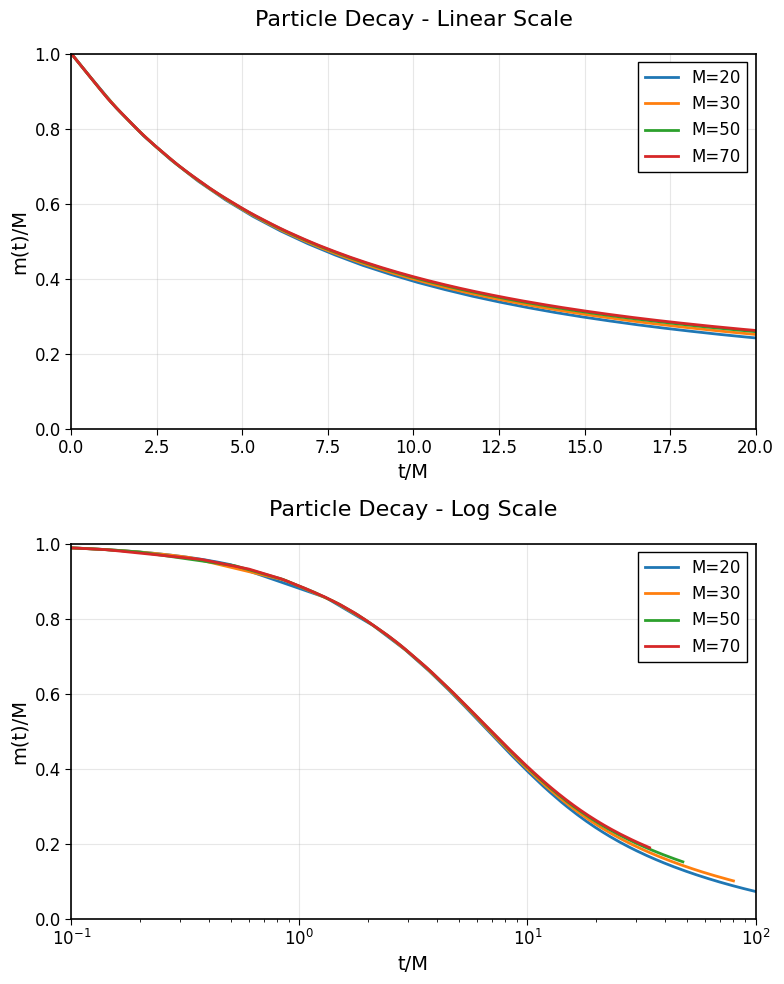
\includegraphics[width=0.7\textwidth]{figures/Fig-3.png}
    \caption{Time evolution of the particle number in the system $\mathcal{S}$ showing exponential decay as particles leak into the environment $\mathcal{E}$. Parameters: $M=20,30,50,70$, $N=10000$, $t_{\mathrm{sys}}=1$, $t_{\mathrm{env}}=4.0$, $g=0.5$.}
    \label{fig:particle_number}
\end{figure}

\subsection{The Page Curve}
Fig. \ref{fig:von_neumann_entropy} displays the central result of this chapter: the time evolution of the von Neumann entanglement entropy. The data clearly exhibits the characteristic "Page curve" behavior—an initial rise followed by a subsequent decay—confirming the expectations discussed in Section \ref{sec:expected_entanglement_dynamics}.

We can identify three distinct regimes:
\begin{enumerate}
    \item \textbf{Linear Growth:} At early times, the entropy grows linearly. This is consistent with the semiclassical picture where entangled particle-hole pairs are produced at the boundary at a constant rate.
    \item \textbf{The Page Time ($t_P$):} The entropy reaches a maximum at a time scale proportional to the system size, $t_P \propto M$. This is the turning point where the system has emitted enough degrees of freedom that the remaining internal states constrain the entanglement.
    \item \textbf{Decay:} At late times, the entropy decreases back toward zero. As the system empties, the dimension of its effective Hilbert space shrinks, forcing the entanglement to vanish.
\end{enumerate}

The maximum entropy scales linearly with system size, $S_{\mathrm{max}} \approx 0.52 M$. It is instructive to compare this to the maximum possible entropy for a system of $M$ qubits, which is $M \ln 2 \approx 0.69 M$. Our value is lower ($0.52 < 0.69$) because our system evolves under free fermion dynamics (Gaussian states), which are not fully ergodic and do not explore the entire Hilbert space like a Haar-random unitary circuit would.

\begin{figure}[H]
    \centering
    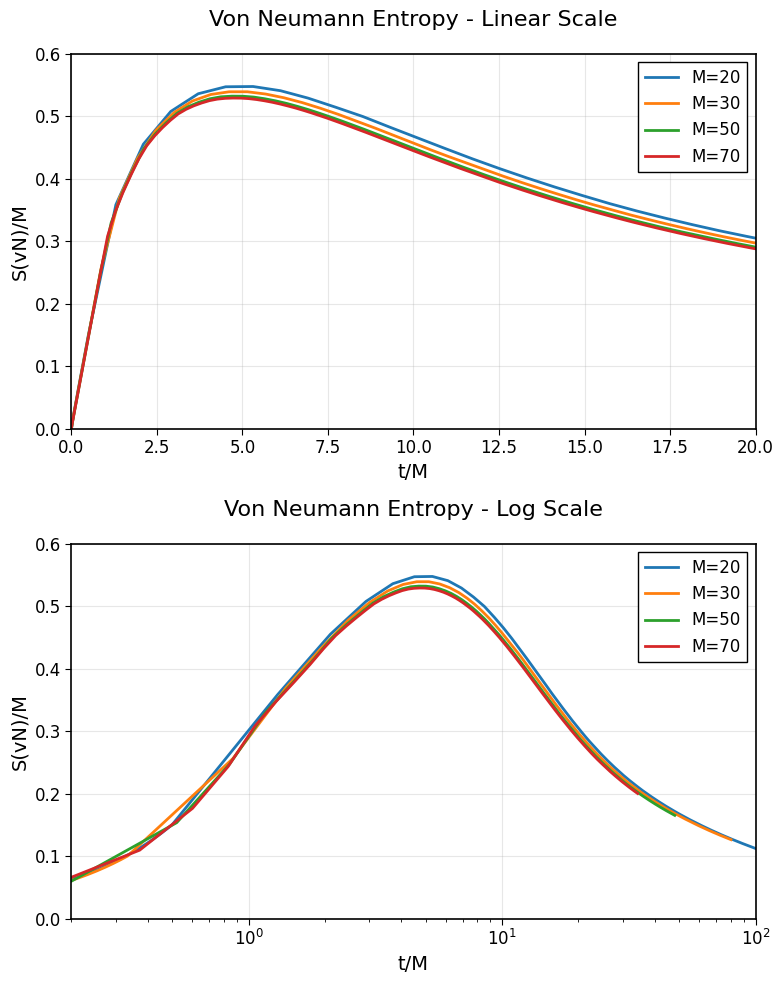
\includegraphics[width=0.7\textwidth]{figures/Fig-4.png}
    \caption{Von Neumann entropy showing Page curve behavior. Parameters: $M=20,30,50,70$, $N=10000$, $t_{\mathrm{sys}}=1.0$, $t_{\mathrm{env}}=4.0$, $g=0.5$.} 
    \label{fig:von_neumann_entropy}
\end{figure}

\subsection{Universality and Scaling}
\label{sec:universality}
Since the decay rate depends on the coupling $g$, the absolute time scale of the dynamics varies with parameters. However, our analytical solution predicts that the physics is universal when viewed in terms of the dimensionless time $\tau$.
An equivalent and physically transparent way to demonstrate this universality is to plot the entanglement entropy against the \emph{fraction of particles emitted}, $1 - m(t)/M$.
Fig. \ref{fig:von_neumann_entropy_g_variation} shows this scaling collapse. The dashed line represents our analytical formula (Eqs. \ref{eq:SvN_continuum} and \ref{eq:nq_tau}).
We observe excellent agreement between the numerical data (solid lines) and the analytical prediction (dashed line) for small couplings (e.g., $g=0.5$). This confirms that the independent RLM approximation captures the essential physics.

\textbf{Finite Environment Effects:}
For larger couplings or late times, we observe deviations where the numerical curves "lift off" from the analytical prediction. This is a finite-size effect of the environment. In our theory, we assumed an infinite bath ($N \to \infty$). In the numerics, the environment is finite ($N=500$).
Each system mode effectively couples to a spectral width $\Gamma_k$ in the environment. If the density of environment states is not high enough, the "infinite bath" assumption breaks down. The residual entropy at late times scales as $(t_{\mathrm{env}}/g)^2 \times (M/N)$, representing the fact that the environment eventually "fills up" or reflects information back to the system.

\begin{figure}[H]
    \centering
    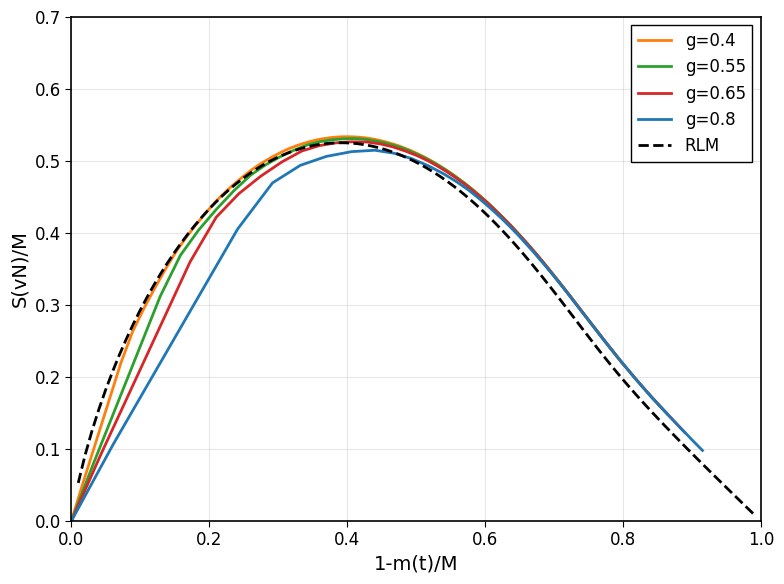
\includegraphics[width=0.7\textwidth]{figures/Fig-5.png}
    \caption{Von Neumann entropy for different values of coupling strength $g$. Parameters: $M=50$, $N=500$, $t_{\mathrm{sys}}=1$, $t_{\mathrm{env}}=5$.}
    \label{fig:von_neumann_entropy_g_variation}
\end{figure}


\section{Interpretation and Generalizations}

\subsection{System Observer Perspective}
From the point of view of an observer in the system $\mathcal{S}$, the dynamical behavior of the entanglement entropy is not
surprising. Initially, system plus environment are in an
unentangled product state \eqref{eq:initial_state}. The process of emitting
particles into the environment generates a complicated
state in the system $\mathcal{S}$ that is entangled with the environment, but ultimately this process continues for so long
that the system $\mathcal{S}$ is driven into a very small effective Hilbert space $\mathcal{H}^{\mathrm{(eff)}}_{\mathrm{sys}} (t \to \infty)$.
Therefore, the entanglement entropy is forced to decrease
again since the asymptotic small effective Hilbert space
does not permit larger values. 

In our model, we have $\mathrm{dim}\, \mathcal{H}^{\mathrm{(eff)}}_{\mathrm{sys}} (t \to \infty)=1$ for $N \gg M^2$ and hence 
$S^{\mathrm{(vN)}} (t \to \infty)=0$.
However, even for smaller ratios
$N/M^2$ one can expect to see Page curve behavior in the
sense that the entanglement entropy decreases after the
Page time, albeit it will not decrease all the way to zero
if $\mathrm{dim}\, \mathcal{H}^{\mathrm{(eff)}}_{\mathrm{sys}} (t \to \infty) > 1$.
Such finite-size behavior is depicted in Fig.~\ref{fig:finite_size_effects} and would be important for experimental realizations where one might not achieve
$N/M^2 \to \infty$.

\begin{figure}[H]
    \centering
    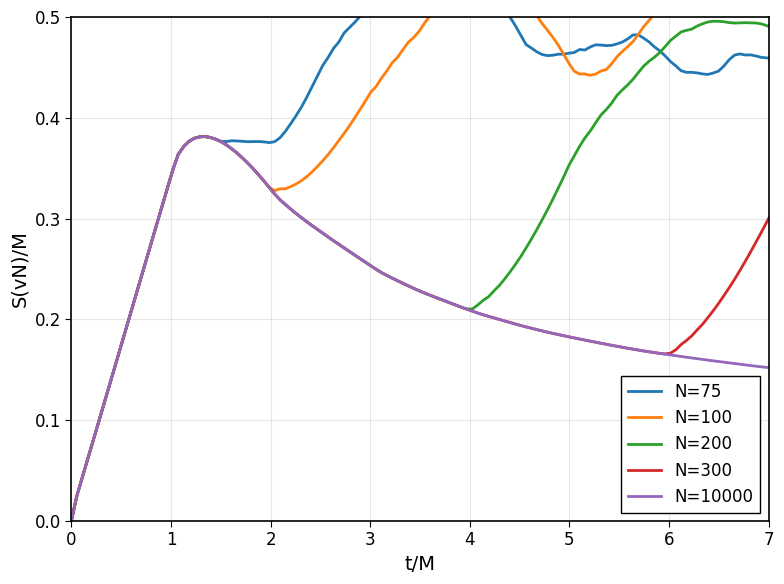
\includegraphics[width=0.7\textwidth]{figures/Fig-6.png}
  \caption{Finite size effects on the entanglement entropy. Parameters: $M=50$, $N= 75, 100, 200, 300, 10000 $, $t_{\mathrm{sys}}=t_{\mathrm{env}}=1$, $g=0.65$.}
  \label{fig:finite_size_effects}
\end{figure}

\subsection{Environment Observer Perspective}
While the decrease of the entanglement entropy after the Page time $t_P$ can be understood from the system point of view, a non-omniscient observer in the environment will find it puzzling: the environment keeps
absorbing particles that have the curious property of reducing its entanglement entropy. This behavior is reminiscent of gas particles carefully reassembling themselves in one half of a gas
cylinder that they were initially released from.

Of course, one can always achieve a decrease of entropy in time-reversal invariant systems by first running time backwards to $-t_0 < 0$ from an initially ordered state $|\Psi(0)\rangle$, and then using this state $|\Psi(-t_0)\rangle$ as the starting point for forward time evolution: In the time interval $[-t_0, 0]$ the entropy then has to decrease. However, this decrease as a function of time is very unstable for generic systems, and even small perturbations will drive the entropy up again. This apparent contradiction between the second law of thermodynamics and microscopic time-reversal invariance was at the center of the Boltzmann--Loschmidt debate, and has been resolved by the understanding of chaotic behavior in generic many-particle systems.

In contrast to such fine-tuned and highly sensitive scenarios, the parameter regime studied here shows a clear and reproducible decrease of the entanglement entropy after the Page time. At the Page time, the entanglement entropy can be made arbitrarily large by increasing $M$. Moderate perturbations that preserve unitary dynamics and do not prevent the net discharge of $\mathcal{S}$ into $\mathcal{E}$ are expected to keep the qualitative rise-and-fall structure, although quantitative features (such as $t_P$ and $S_{\max}$) can shift. An observer limited to the environment, with no knowledge of the full initial state, would interpret such robust late-time entropy decrease as strongly time-asymmetric behavior.

In this model, the dynamical buildup of long-range entanglement between $\mathcal{H}_{\mathrm{sys}}$ and $\mathcal{H}_{\mathrm{env}}$ up to the Page time is responsible for the Page-curve behavior: particles emitted into the environment after the Page time carry entanglement across the boundary, leading to the bending down of the curve. This mechanism persists within the validity regime discussed in Section~\ref{subsec:validity_conditions}.

\subsection{Breakdown of the Semiclassical Picture}
At early times, the entanglement entropy grows linearly at a rate proportional to the particle current:
\begin{equation}
\frac{dS^{(\mathrm{vN})}}{dt} \propto |I(t)|
\label{eq:semiclassical_relation}
\end{equation}
This semiclassical relation, where each tunneling particle contributes a fixed amount of entanglement, is consistent with the quasiparticle picture of entanglement spreading~\cite{Calabrese_2005}.

However, this simple relation must break down at the Page time. As shown in Fig.~\ref{fig:particle_number}, the particle current $I(t) = \dot{m}(t)$ remains smooth and featureless across the Page time---there is no discernible signature at $t = t_P$. Yet the entanglement entropy reaches its maximum and begins to decrease. This demonstrates that the Page curve is a phenomenon of \emph{quantum information} that is invisible to local observables like particle number or current.

The breakdown of the semiclassical picture can be understood as follows: At early times, particles tunneling into the environment carry ``fresh'' entanglement with the system. After the Page time, the system has evolved to a sufficiently complex state that additional particle emission actually \emph{reduces} the entanglement. The emitted particles are now anti-correlated with the previously emitted particles in a way that purifies the environment state.

\subsection{Generalizations}
The key mechanism driving the Page curve in our model---the progressive reduction of the system's effective Hilbert space dimension as it discharges particles---does not rely on the specific free-fermion structure. This suggests that Page-curve-like entanglement dynamics should arise in a broader class of open quantum systems, provided that
(i) the system--environment coupling drives the system toward a low-dimensional subspace, and
(ii) the total evolution is unitary.
We briefly note the most natural extensions here; a detailed discussion is given in Section~\ref{sec:future_work}.

\paragraph{Interacting systems.} The effective Hilbert space shrinking mechanism is kinematic and independent of integrability. For interacting systems, one therefore expects similar qualitative Page-curve behavior, though the quantitative features---such as the entropy scaling and the Page time---may differ because interactions can thermalize the system and alter the entanglement structure. Numerical access would be limited to smaller system sizes due to the absence of Gaussian-state simplifications.

\paragraph{Higher dimensions and other geometries.} The essential physics (particle transfer leading to effective Hilbert space reduction) extends to higher-dimensional systems where a finite region is coupled to a large bath, as well as to alternative coupling geometries such as bulk coupling or multi-lead setups.

\paragraph{Connection to black hole physics.}
Our model illustrates an analogy to Polchinski's ``burning piece of coal''~\cite{Polchinski_2016}: The early photons (particles emitted before the Page time) are entangled with the remaining coal (system), but when the coal has burned completely, the outgoing photons must be in a pure state (assuming the coal was initially in a pure state). While this is fundamentally different from a black hole due to the lack of an event horizon, the qualitative Page curve behavior---initial entanglement growth followed by purification---is the same.

\begin{remark}
The original analysis in Ref.~\cite{Kehrein_2024} also investigates the min-entropy (the $q \to \infty$ limit of the Rényi entropy) and identifies a quantum phase transition in the entanglement Hamiltonian that slightly precedes the Page time. Additionally, the paper shows that the energy variance of the environment Hamiltonian, $\Delta H_{\mathrm{env}}^2(t)$, exhibits analogous Page-curve-like behavior---increasing until the Page time and then decreasing as the system empties. These features provide additional signatures of the Page curve dynamics but are beyond the scope of the present thesis.
\end{remark}

\chapter{Conclusion}
\label{ch:conclusion}

This thesis investigated entanglement dynamics in an open quantum many-body system: a one-dimensional free-fermion chain coupled to a large environment.
The central result is that this simple and exactly solvable model exhibits clear Page-curve-like behavior in its entanglement entropy dynamics.

\section{Summary of Findings}
\label{sec:summary}

The main results are:

\paragraph{Model and Physical Setup.}
We studied a tight-binding fermionic chain of $M$ sites (the system $\mathcal{S}$) weakly coupled at one boundary to a much larger chain of $N \gg M$ sites (the environment $\mathcal{E}$). The initial state consists of a fully occupied system and an empty environment, creating a particle imbalance that drives the subsequent dynamics.

\paragraph{Numerical Solution via Correlation Matrix Formalism.}
Using the Peschel formalism, we showed that for free fermion systems, the entanglement entropy can be computed efficiently from the eigenvalues of the restricted correlation matrix $C_{\mathcal{S}}(t)$. This reduces the computational complexity from exponential (tracking the full $2^M \times 2^M$ density matrix) to polynomial scaling ($M \times M$ matrix operations), enabling simulations for systems with tens of sites.

\paragraph{Analytical Solution via Resonant Level Model Factorization.}
In the weak-coupling limit ($g \ll \sqrt{t_{\mathrm{sys}} t_{\mathrm{env}}}$), we derived a controlled analytical description by showing that, within Born--Markov/secular approximations, the many-body dynamics factorizes into $M$ independent resonant level models (RLMs). Each momentum mode $k$ of the system couples to a disjoint spectral window of the environment, allowing the reduced density matrix to be written as a tensor product:
\begin{equation}
\rho_{\mathrm{sys}}(t) = \bigotimes_{k=1}^M \rho_k^{(\mathrm{RLM})}(t)
\end{equation}
This factorization leads to exponential decay of mode occupations with mode-dependent decay rates $\Gamma_k \propto \sin^2(\pi k/(M+1))$.

\paragraph{Page Curve Dynamics.}
We confirmed that the entanglement entropy exhibits the characteristic Page curve behavior:
\begin{enumerate}
\item \textbf{Linear growth} at early times, driven by particle-hole pair production at the system-environment boundary;
\item \textbf{Maximum entropy} at the Page time $t_P \propto M$, where $S_{\mathrm{max}} \approx 0.52 M$. This is lower than the absolute maximum of $M \ln 2 \approx 0.69 M$ for $M$ fermionic modes, reflecting the fact that free-fermion (Gaussian-state) dynamics are not fully ergodic and do not explore the entire Hilbert space;
\item \textbf{Decay} at late times as the system empties and its effective Hilbert space dimension shrinks.
\end{enumerate}

\paragraph{Universal Scaling.}
In the continuum limit ($M \gg 1$), we showed that the dynamics depend only on the dimensionless time $\tau = 4g^2 t / [(M+1) t_{\mathrm{env}}]$ and continuous momentum $q$. When plotted against the fraction of emitted particles, all systems in the appropriate parameter regime collapse onto a single universal curve, independent of microscopic parameters.

\paragraph{Numerical Validation.}
The analytical predictions were validated against numerical simulations using the correlation-matrix formalism.
Excellent agreement is observed in the weak-coupling regime, with deviations appearing mainly at late times due to finite environment size effects.

\section{Future Work}
\label{sec:future_work}

Several natural extensions of this work merit further investigation:

\paragraph{Bosonic Systems.}
An important direction is to extend the analysis to bosonic systems, such as a chain of coupled harmonic oscillators or the spin-boson model. While these systems lack an analytical solution comparable to the fermionic RLM factorization, numerical methods based on covariance matrices (the bosonic analog of the Peschel formalism) could be employed. Preliminary considerations suggest that similar Page-curve-like behavior should emerge, though the absence of the Pauli exclusion principle may lead to quantitative differences in the entropy scaling.

\paragraph{Interacting Systems.}
Our analysis relied on the quadratic (free) nature of the Hamiltonian. Extending to interacting fermions would break the Gaussian state structure and require more sophisticated techniques such as tensor network methods (DMRG, TEBD) or quantum Monte Carlo. The key question is whether the Page curve phenomenology survives in the presence of interactions, and if so, how the Page time and maximum entropy scale with interaction strength.

\paragraph{Different Coupling Geometries.}
We considered boundary coupling between system and environment. Alternative geometries---such as bulk coupling at multiple sites, or coupling to multiple independent environments---could reveal different entanglement dynamics. In particular, coupling at both ends of the chain might lead to qualitatively different behavior due to interference effects between the two boundaries.

\paragraph{Finite Temperature Effects.}
Our analysis assumed a zero-temperature initial state (empty environment). At finite temperature, the environment contains thermal excitations that can tunnel into the system, potentially leading to equilibration rather than complete emptying. The interplay between thermal fluctuations and quantum entanglement in this setting deserves further study.

\paragraph{Experimental Realizations.}
Cold atom systems in optical lattices provide a natural platform for realizing the model studied here. The weak-coupling limit corresponds to a tunnel barrier between two lattice regions. Modern quantum gas microscopes allow single-site-resolved measurements of particle distributions, enabling direct observation of the particle number decay $m(t)$. Measuring entanglement entropy experimentally remains challenging but may be accessible through randomized measurement protocols or by measuring R\'enyi entropies via interference experiments.

\section{Broader Implications}
\label{sec:implications}

The results of this thesis connect to several broader themes in modern physics:

\paragraph{Black Hole Information Paradox.}
The Page curve was originally introduced in the context of black hole evaporation, where it describes how the entanglement entropy of Hawking radiation should evolve if information is preserved. Our fermionic model provides a simple, exactly solvable analog where the system (black hole) emits particles into the environment (radiation) with qualitatively similar entanglement dynamics. While our model lacks the gravitational complexity of actual black holes, it shows that Page-curve-like behavior can emerge in simple open quantum systems with suitable initial conditions.

\paragraph{Quantum Thermalization.}
The Page-curve dynamics illustrate information exchange and relaxation in an open quantum system. The initial growth of entanglement corresponds to spreading of correlations across the system-environment boundary, while the late-time decay reflects the reduction of accessible subsystem degrees of freedom as the system empties. Although this free-fermion setup is not a direct test of the eigenstate thermalization hypothesis, it provides an analytically controlled benchmark for open-system entanglement dynamics.

\paragraph{Quantum Information Processing.}
Understanding entanglement dynamics in open systems is relevant to quantum error correction and fault-tolerant quantum computing. The timescales identified here---particularly the Page time and mode-dependent decay rates---illustrate how quantum information leaks from a finite system into its environment. While our free-fermion model is too idealized to set direct engineering constraints, the analytical expressions relating these timescales to system parameters may offer qualitative guidance for understanding decoherence in weakly coupled quantum devices.

\paragraph{Condensed Matter Physics.}
Free fermion models with boundary dissipation appear naturally in the study of quantum transport, mesoscopic physics, and non-equilibrium steady states. The correlation matrix formalism developed here provides efficient numerical tools for studying entanglement in such systems. The factorization into independent resonant level models may have applications beyond entanglement, such as in understanding transport coefficients or spectral functions in weakly coupled systems.

In conclusion, this thesis shows that the Page curve---a concept originally developed in black hole physics---emerges naturally in a simple, exactly solvable condensed-matter setting.
The analytical and numerical framework developed here provides a foundation for studying entanglement dynamics in more complex open quantum many-body systems.

% Back matter
% Note: report class doesn't have \backmatter
\cleardoublepage

% Bibliography with proper spacing
\cleardoublepage
\phantomsection
\addcontentsline{toc}{chapter}{Bibliography}
\printbibliography[title=Bibliography]

% Appendices
\appendix
\phantomsection
\addcontentsline{toc}{chapter}{Appendices}

\chapter{Mathematical Derivations}
\label{app:derivations}

\section{Surface Green's function and local DOS at a boundary}
\label{app:surface_gf}
Here we derive the boundary (surface) retarded Green's function $g^{R}_{11}(E)$ and the corresponding local density of states (DOS) for a semi-infinite tight-binding chain with hopping $t_{\mathrm{env}}$:
\begin{equation}
 H_{\mathrm{env}} = -t_{\mathrm{env}} \sum_{n\ge 1} \big( |n\rangle\langle n{+}1| + |n{+}1\rangle\langle n| \big).
\end{equation}
Define the retarded Green's function $G^{R}(E) = (E + i0^{+} - H_{\mathrm{env}})^{-1}$ and the surface element $g^{R}_{11}(E) = \langle 1| G^{R}(E) |1\rangle$.

\paragraph{Recursive (decimation) derivation.}
Partition the Hilbert space into site $|1\rangle$ and the rest $\mathcal{H}_{\ge 2}$ (sites $n\ge 2$). The coupling between them is $-t_{\mathrm{env}} (|1\rangle\langle 2| + |2\rangle\langle 1|)$. The Dyson equation yields
\begin{equation}
 g^{R}_{11}(E) = \frac{1}{E + i0^{+} - \Sigma^{R}(E)}\,, \qquad \Sigma^{R}(E) = t_{\mathrm{env}}^{2}\, g^{R}_{22;(\ge 2)}(E),
\end{equation}
where $g^{R}_{22;(\ge 2)}$ is the $(2,2)$ element of the Green's function for the semi-infinite subchain starting at site $2$. By translational invariance away from the boundary, $g^{R}_{22;(\ge 2)}(E) = g^{R}_{11}(E)$. Therefore $g(E) \equiv g^{R}_{11}(E)$ obeys the quadratic equation
\begin{equation}
 t_{\mathrm{env}}^{2} g^{2} - (E + i0^{+}) g + 1 = 0.
 \label{app:eq:quad_g}
\end{equation}
Solving and selecting the retarded (causal) branch with $\mathrm{Im}\,g^{R}_{11}(E)<0$ gives, for $|E|<2 t_{\mathrm{env}}$,
\begin{equation}
 g^{R}_{11}(E) = \frac{E - i\sqrt{4 t_{\mathrm{env}}^{2} - E^{2}}}{2 t_{\mathrm{env}}^{2}}\,.
 \label{app:eq:surface_gf}
\end{equation}
For $|E|>2 t_{\mathrm{env}}$ the square root is real and $g^{R}_{11}(E)$ is real (no spectral weight).

\paragraph{Local DOS.}
The local DOS at the boundary is
\begin{equation}
 \rho_{\mathrm{loc}}(E) = -\frac{1}{\pi} \, \mathrm{Im}\, g^{R}_{11}(E)
 = \frac{1}{2\pi} \, \frac{\sqrt{4 t_{\mathrm{env}}^{2} - E^{2}}}{t_{\mathrm{env}}^{2}}\,, \qquad (|E|<2 t_{\mathrm{env}}).
 \label{app:eq:rho_loc}
\end{equation}
In particular, at the band center $E=0$ one finds $\rho_{\mathrm{loc}}(0) = 1/(\pi t_{\mathrm{env}})$. These results coincide with Eqs.~\eqref{eq:surface_GF} and~\eqref{eq:rho_loc} used in the main text to obtain the level width $\Gamma_k$ and the decay laws in the wide-band limit.

\section{Discrete Sine Sum Identity}
\label{app:sine_identity}

We prove the identity used in the normalization of the eigenfunctions:
\begin{equation}
\sum_{i=1}^M \sin^2\left(\frac{\pi k i}{M+1}\right) = \frac{M+1}{2}
\end{equation}
for integer $k \in \{1, 2, \ldots, M\}$.

Using the identity $\sin^2\theta = \frac{1}{2}(1 - \cos 2\theta)$:
\begin{align}
\sum_{i=1}^M \sin^2\left(\frac{\pi k i}{M+1}\right) &= \frac{1}{2}\sum_{i=1}^M \left[1 - \cos\left(\frac{2\pi k i}{M+1}\right)\right] \nonumber\\
&= \frac{M}{2} - \frac{1}{2}\sum_{i=1}^M \cos\left(\frac{2\pi k i}{M+1}\right)
\end{align}

The sum over cosines is the real part of a geometric series. Define $\omega = e^{2\pi i k/(M+1)}$, which is a primitive $(M+1)$-th root of unity when $k \in \{1, \ldots, M\}$. Then:
\begin{equation}
\sum_{i=1}^M \omega^i = \omega \cdot \frac{1 - \omega^M}{1 - \omega} = \omega \cdot \frac{1 - \omega^{-1}}{1 - \omega} = -1
\end{equation}
where we used $\omega^{M+1} = 1$, hence $\omega^M = \omega^{-1}$.

Alternatively, the sum of all $(M+1)$-th roots of unity vanishes: $\sum_{i=0}^{M} \omega^i = 0$. Since the $i=0$ term equals 1, we have $\sum_{i=1}^M \omega^i = -1$.

Taking the real part: $\sum_{i=1}^M \cos(2\pi k i/(M+1)) = -1$. Therefore:
\begin{equation}
\sum_{i=1}^M \sin^2\left(\frac{\pi k i}{M+1}\right) = \frac{M}{2} - \frac{1}{2}(-1) = \frac{M+1}{2}
\end{equation}
as claimed.


\chapter{Simulation Code}
\label{app:code}

This appendix contains the core Python code used for all numerical simulations presented in this thesis. The implementation is based on the correlation-matrix formalism described in Chapter \ref{ch:fermionic}.

\section{Numerical Simulation Class}
\label{app:code:simulation}

The \texttt{PageCurveSimulation} class implements the full numerical pipeline: Hamiltonian construction, diagonalization, time evolution of the correlation matrix, and computation of entanglement measures.

\begin{lstlisting}[caption={Core simulation class for the fermionic Page curve model.}]
import numpy as np
from scipy.linalg import eigh
from scipy.integrate import quad
from tqdm import tqdm

class PageCurveSimulation:
    def __init__(self, M, N, g, t_sys=1.0, t_env=4.0):
        """
        Initialize the Page Curve simulation parameters.
        M: system size (number of system sites)
        N: environment size (number of environment sites)
        g: coupling strength between system and environment
        t_sys: hopping parameter in system
        t_env: hopping parameter in environment
        """
        self.M = M
        self.N = N
        self.total_sites = M + N
        self.g = g
        self.t_sys = t_sys
        self.t_env = t_env
        self.H = None
        self.eigenvalues = None
        self.eigenvectors = None
        self.C0 = None

    def hamiltonian(self):
        """Construct the full Hamiltonian matrix."""
        H = np.zeros((self.total_sites, self.total_sites))
        # System hopping (sites 0 to M-1)
        for i in range(self.M - 1):
            H[i, i+1] = -self.t_sys
            H[i+1, i] = -self.t_sys
        # Environment hopping (sites M to M+N-1)
        for i in range(self.M, self.total_sites - 1):
            H[i, i+1] = -self.t_env
            H[i+1, i] = -self.t_env
        # System-environment coupling at boundary.
        # The coupling is placed at the last system site (index M-1)
        # and the first environment site (index M). This is physically
        # equivalent to coupling at site 1: |psi_k(1)|^2 = |psi_k(M)|^2
        # for open BC, due to the reflection symmetry sin(pi*k*i/(M+1))
        # = sin(pi*k*(M+1-i)/(M+1)) of the eigenfunctions.
        # The sign -g here is conventional; the observable physics
        # (decay rates Gamma_k) depends only on g^2, so g -> -g
        # leaves all entanglement dynamics unchanged.
        H[self.M-1, self.M] = -self.g
        H[self.M, self.M-1] = -self.g
        self.H = H
        return H

    def diagonalize_hamiltonian(self):
        """Diagonalize the Hamiltonian."""
        if self.H is None:
            self.hamiltonian()
        self.eigenvalues, self.eigenvectors = eigh(self.H)
        return self.eigenvalues, self.eigenvectors

    def setup_initial_state(self):
        """Setup initial correlation matrix:
        system filled, environment empty."""
        C0 = np.zeros((self.total_sites, self.total_sites))
        for i in range(self.M):
            C0[i, i] = 1.0
        self.C0 = C0
        return C0

    def evolve_correlation_matrix(self, t):
        """Time evolve the correlation matrix to time t.
        C(t) = U(t) C(0) U^dag(t)"""
        if self.eigenvalues is None:
            self.diagonalize_hamiltonian()
        if self.C0 is None:
            self.setup_initial_state()
        time_phases = np.exp(-1j * self.eigenvalues * t)
        U_t = (self.eigenvectors
               @ np.diag(time_phases)
               @ self.eigenvectors.T.conj())
        C_t = U_t @ self.C0 @ U_t.T.conj()
        return C_t

    def extract_system_correlation_matrix(self, C_t):
        """Extract the M x M system block."""
        return C_t[:self.M, :self.M]

    def particle_number(self, C_sys):
        """Particle number in the system."""
        return np.trace(C_sys).real

    def von_neumann_entropy(self, C_sys):
        """Von Neumann entropy from correlation matrix
        eigenvalues."""
        eigenvals = np.linalg.eigvalsh(C_sys)
        eigenvals = eigenvals[
            (eigenvals > 1e-12) & (eigenvals < 1 - 1e-12)
        ]
        return -np.sum(
            eigenvals * np.log(eigenvals)
            + (1 - eigenvals) * np.log(1 - eigenvals)
        )

    def purity(self, C_sys):
        """Purity S(2) = -log(Tr[rho^2])."""
        eigenvals = np.real(np.linalg.eigvalsh(C_sys))
        eigenvals = eigenvals[eigenvals > 1e-12]
        purity_val = -np.log(
            eigenvals**2 + (1 - eigenvals)**2
        )
        return np.sum(purity_val)

    def min_entropy(self, C_sys):
        """Min-entropy S(min)."""
        eigenvals = np.real(np.linalg.eigvalsh(C_sys))
        eigenvals = eigenvals[
            (eigenvals > 1e-12) & (eigenvals < 1 - 1e-12)
        ]
        return np.sum(
            -2 * np.log(np.maximum(eigenvals, 1 - eigenvals))
        )

    def energy_variance(self, C_t):
        """Energy variance w.r.t. environment Hamiltonian."""
        C_env = C_t[self.M:, self.M:]
        H_env = np.zeros((self.N, self.N))
        for i in range(self.N - 1):
            H_env[i, i+1] = -self.t_env
            H_env[i+1, i] = -self.t_env
        H_exp = np.trace(C_env @ H_env).real
        H2_exp = np.trace(C_env @ H_env @ H_env).real
        return H2_exp - H_exp**2

    def run_simulation(self, times):
        """Run for an array of times; return
        particle numbers, entropies, purities,
        min-entropies, and energy variances."""
        particles, entropies = [], []
        purities, min_ents, variances = [], [], []
        for t in tqdm(times, desc="Time evolution"):
            C_t = self.evolve_correlation_matrix(t)
            C_sys = self.extract_system_correlation_matrix(C_t)
            particles.append(self.particle_number(C_sys))
            entropies.append(self.von_neumann_entropy(C_sys))
            purities.append(self.purity(C_sys))
            min_ents.append(self.min_entropy(C_sys))
            variances.append(self.energy_variance(C_t))
        return (np.array(particles), np.array(entropies),
                np.array(purities), np.array(min_ents),
                np.array(variances))
\end{lstlisting}

\section{Analytical Predictions}
\label{app:code:analytical}

The \texttt{AnalyticalPageCurve} class evaluates the weak-coupling analytical expressions derived in Section~\ref{sec:analytical_solution} using numerical quadrature.

\begin{lstlisting}[caption={Analytical Page curve predictions from the disjoint resonant level model.}]
from scipy.integrate import quad

class AnalyticalPageCurve:

    @staticmethod
    def analytical_particle_number(tau):
        """Analytical particle fraction m(tau)/M
        from Eq. (23)."""
        def integrand(k):
            return np.exp(-tau * np.sin(k)**2)
        result, _ = quad(integrand, 0, np.pi)
        return result / np.pi

    @staticmethod
    def analytical_von_neumann_entropy(tau):
        """Analytical von Neumann entropy per site
        from Eqs. (24)--(26)."""
        def integrand(k):
            n_k = np.exp(-tau * np.sin(k)**2)
            n_k = np.clip(n_k, 1e-15, 1 - 1e-15)
            return -(n_k * np.log(n_k)
                     + (1 - n_k) * np.log(1 - n_k))
        result, _ = quad(integrand, 0, np.pi)
        return result / np.pi

    @staticmethod
    def analytical_purity(tau):
        """Analytical purity S(2) per site."""
        def integrand(k):
            n_k = np.exp(-tau * np.sin(k)**2)
            return n_k**2 + (1 - n_k)**2
        result, _ = quad(integrand, 0, np.pi)
        return -np.log(result / np.pi)

    @staticmethod
    def analytical_min_entropy(tau):
        """Analytical min-entropy S(min) per site."""
        def integrand(k):
            n_k = np.exp(-tau * np.sin(k)**2)
            return -np.log(np.maximum(n_k, 1 - n_k))
        result, _ = quad(integrand, 0, np.pi)
        return 2 * result / np.pi

    @staticmethod
    def analytical_energy_variance(tau, t_env=4.0):
        """Analytical energy variance from Eq. (B4)."""
        def integrand(k):
            n_k = np.exp(-tau * np.sin(k)**2)
            return np.sin(k)**2 * n_k * (1 - n_k)
        result, _ = quad(integrand, 0, np.pi)
        return (2 * t_env**2 / np.pi) * result
\end{lstlisting}

\section{Usage Example}
\label{app:code:usage}

The following snippet illustrates how the classes above are used to generate the Page curve data presented in the main text.

\begin{lstlisting}[caption={Example: computing the Page curve for several system sizes.}]
import numpy as np
import matplotlib.pyplot as plt

M_values = [25, 35, 50, 75]
N = 10000
g = 0.5

for M in M_values:
    sim = PageCurveSimulation(M, N, g,
                              t_sys=1.0, t_env=4.0)
    times = np.linspace(0, 200, 200)
    particles, entropies, _, _, _ = (
        sim.run_simulation(times)
    )
    # Rescaled Page curve
    plt.plot(times / M, entropies / M,
             label=f'M={M}')

plt.xlabel('t / M')
plt.ylabel(r'$S_{\mathrm{vN}} / M$')
plt.legend()
plt.show()
\end{lstlisting}

\end{document}
